\subsection{Data Sets}
\label{sec:data_sets}

Experimental evaluations are conducted on three data sets: Halo 2 XBox Live
matches, Australian Football
(Rugby) League (AFL)%\footnote{\noindent
%  \url{http://www.csse.monash.edu.au/~footy/data/index.shtml}}
and UK
Premier League (UK-PL)\footnote{\noindent \url{http://www.football-data.co.uk/englandm.php}}.  The Halo 2 data consists of a
set of match outcomes comprising 6227 games for 1672 players. We note there are negative scores for this data, so we add the absolute value of the minimal score to all scores to use the data with all proposed models.

The training and testing settings are described as follows.  For Halo
2~\footnote{\noindent Credit for the use of the Halo 2 Beta Data set
is given to Microsoft Research Ltd. and Bungie.}, the last 10\%
of matches are used for testing, and we use different proportions of
the first 90\% of data for training. There are 8 proportions used
for training, ranging from 10\% to 80\% with an increment of
10\%, and 90\% is not used for training due to cross validation. To cross validate, we randomly sample the data and run the learning 10 times at each proportion level
to get standard error bars. Note that there are some players in the
testing games who are not involved in any training data sets,
particularly when small proportion of training data set is selected
(e.g., the first 10 percent games); we remove these games in the
testing set when reporting performances for all models.

For both UK-PL and AFL datasets, cross validation is performed by
training and testing for each year separately (14 years for UK-PL, and
11 years for AFL).  For these two datasets, we test the last 20\%
percent of matches in each year, with the training data increasing
incrementally from 10\% to 80\% of the initial matches.

\subsection{Evaluation Criteria}

We evaluate performances using three criteria: {\it information gain}
of predicting winning probability of a team
(Section~\ref{sec:informationGain}),
{\it win/lose prediction accuracy}
(Section~\ref{sec:WLPredictionAccuracy}), {\it win/lose/draw prediction accuracy} (Section~\ref{sec:multiclassClassification}), 
and {\it score prediction errors}
(Section~\ref{sec:scorePredictionError}).
While the first three criteria focus on predicting win/lose or win/lose/draw, the fourth
criterion measures how good a model is at predicting scores, for which
TrueSkill does not apply since it is restricted to WLD only. Let us
introduce each criterion in detail.

\subsubsection{Information Gain}
\label{sec:informationGain}

The first criterion we use to evaluate different approaches is
\emph{information gain}, which is proposed in the \emph{Probabilistic Footy
Tipping Competition}\footnote{Refer to
\url{http://www.csse.monash.edu.au/~footy/}}: if a predictor assigns
probability $p$ to team $i$ winning, then the score (in ``bits")
gained is $1+\log_2(p)$ if team $i$ wins, $1+\log_2(1-p)$ if team $i$ loses, $1+(1/2)\log_2(p(1-p))$ if draw happens.
This evaluation metric can be viewed as an information gain
interpretable variant of a log likelihood score where an uninformed
prediction of $p=0.5$ leads to a score of 0 and a definite prediction
of $p=1$ ($p=0$) leads to a score of $-\infty$ if predicting
incorrectly and 1 if predicting correctly.
In Section~\ref{sec:inference}, we showed how to compute the win
probability $p$ for each model.

\subsubsection{Win/no-Win Prediction Accuracy}
\label{sec:WLPredictionAccuracy}

While information gain provides a sense of how well the models fit the
data, it is also interesting to see how accurate the models were at
predicting match outcomes in terms of win/no-win (e.g., loss/draw).  To compare
classification performance of each model, we report the
win/not winning prediction accuracy in terms of area under the curve (AUC) for the
games with a win or loss outcome. 

%This is a straighforward metric to
%evaluate in expectation: for the univariate skill models we simply
%assign a win to the team with the higher mean skill level, for the
%remaining offence/defence score models, we simply assign a win to the
%team with the higher expected score (these simple calculations are
%explained in the next subsection).

%It is essential to evaluate the prediction accuracy in terms of
%win/loss for matchmaking. To describe this evaluation criterion, let
%us first introduce when a model predicts team $i$ winning, in a match
%with team $j$. Based on the belief of a model, its prediction is
%correct: either (1) team $i$'s mean skill is larger than that of team
%$j$ skill and team $i$ wins, or (2) team $i$'s mean skill is smaller
%than that of team $j$ skill and team $i$ loses. Suppose there are $M$
%matches, and the model predicts correctly for $N$ times, then the
%prediction accuracy is $N/M$.

\subsubsection{Multi-Class Classification Among Win, Lose, and Draw}
\label{sec:multiclassClassification}
The Win/no-Win prediction accuracy introduced above suits for binary classification. This criterion does not necessarily apply to the cases where draws can happen such as a match outcomes end up with each team obtaining 3 goals in football games. To accommodate the applications where draws can happen, we evaluate the predictive performance in terms of a multi-class classification problem where there are three classes for a game: winning, drawing, and losing for one out of the two teams participating in two-team game. We use the Brier score introduced in~\cite{Brier:BrierScore} as a performance measure for this multi-class classification setting, as in~\cite{huang06GeneralizedBradleyTerryModels}. 

Following~\cite{huang06GeneralizedBradleyTerryModels}, we define the Brier Score for a set of $N$ testing games below:
\begin{align}
	\frac{1}{N}\sum_{i=1}^{N}\left( \sum_{k=1}^{K} \left(\mathbb{I}[y_i = k] - \hat{p}_{k}^{i}\right)^2  \right),
\end{align}
where $\hat{p}_{k}^{i}$ is the probability estimate of the $i$th game being assigned to the $k$-th class, and $I(y_i = k)$ is an indicator function (1 if $y_i=k$ and 0 otherwise). Note that one advantage of this measurement is that it does not require the true probability of a data point belonging to a class. 

\subsubsection{Score Prediction Error}
\label{sec:scorePredictionError}

%We evaluate the score prediction accuracy for the two full
% score prediction models: Poisson-OD and Gaussian-OD.
%For the Poisson-OD model (Figure~\ref{fig:trueskill_variant}), the
%expected score for team $i$ ($j$) is $\exp(x)$ ($\exp(y)$) and for the
%Gaussian-OD model
%(Figure~\ref{fig:modelAndInferenceGaussianGraphicalModel}), the
%expected score for team $i$ ($j$) is $x$ ($y$), where $x$ ($y$) is the
%difference in mean performances giving $s_i$ ($s_j$).  The Gaussian-SD model
%(Figure~\ref{fig:modelAndInferenceGaussianGraphicalModelScoreDifference}),
%directly produces \emph{score difference} predictions $d = s_i - s_j$,
%which is just the difference in mean performances of the two teams.
%Because scores for different games have a different scale, we introduce
%a relative measure of score accuracy.
%Suppose $s^*$ is the true score, and
%$\hat{s}$ the expected score. We define the
%relative score prediction error $e(s^*, \hat{s})$ as
%\begin{align}
%e(s^*, \hat{s})= \frac{|\hat{s}-s^*|}{|s^*|}.
%\end{align}
%%Therefore, the larger the deviation of $\hat{s}$ to the true score $s^*$, the larger the error.
%Note that the prediction error can be larger than one,
%e.g. $\hat{s}=5, s^*=2$ causing $e(s^*, \hat{s})=1.5$.




%For the Poisson-OD model (Figure~\ref{fig:trueskill_variant}), the
%expected score for team $i$ ($j$) is $\exp(x)$ ($\exp(y)$) and for the
%Gaussian-OD model
%(Figure~\ref{fig:modelAndInferenceGaussianGraphicalModel}), the
%expected score for team $i$ ($j$) is $x$ ($y$), where $x$ ($y$) is the
%difference in mean performances giving $s_i$ ($s_j$).  The Gaussian-SD model
%(Figure~\ref{fig:modelAndInferenceGaussianGraphicalModelScoreDifference}),
%directly produces \emph{score difference} predictions $d = s_i - s_j$,
%which is just the difference in mean performances of the two teams.
We evaluate the score prediction accuracy for Poisson-OD and
Gaussian-OD models for \emph{each} team in terms of the mean absolute
error (MAE), defined as below:
\begin{align}
    \frac{1}{2N} \sum_{i=1}^{2N} \left(| \hat{s_i} - s_i | + \hat{s_j} - s_j |\right)
\end{align}
where $\hat{s_i}$ ($\hat{s_j}$) is the predicted score for team $i$ ($j$), $s_i$ ($s_j$) the ground truth, and $N$ the number of two-team matches for with teams indexed by $i$ and $j$. 

Note that we must omit the Gaussian-SD model since it can only predict score differences rather than scores. To benchmark the score prediction performance of the Poisson-OD and Gaussian-OD models, we compare with an average score prediction methods. This average score methods simply use the average scores for a team computed from the training games as predictions for testing games.

\subsection{Results on Four Criteria}
\label{sec:results}

Experimental results are reported according to the parameter
configurations shown in Table~\ref{table:Parameters}. Parameters for the slice sampling used in the Poisson-OD model include the burn-in, thinning, and the number of samples required, which we set to 1000, 5, and 1000, respectively. 
Now we discuss the results against these four criteria on three real data sets below. 
\begin{table}[htbp!]
\caption{Parameter settings. Priors on offence/defence skills: $\mathcal{N}(\mu_{0},\sigma_{0}^2)$ with $\mu_{0}=25$ and $\sigma_{0}=25/3$. Performance variance: $\beta$, $\beta_o$, $\beta_d$.}
\begin{center}
\small
\begin{tabular}{cc}
  \hline
  Model             & Parameter ($\epsilon,\gamma$ empirically estimated)\\
  \hline
  TrueSkill          & $\beta=\sigma_{0}/2$, $\epsilon$: draw probability\\
  Poisson-OD(VB)         & $\beta_o=\beta_d=\sigma_{0}/2$\\
  Poisson-OD(Sampling)         & $\beta_o=\beta_d=\sigma_{0}/2$\\
  Gaussian-OD    & $\beta_o=\beta_d=\sigma_{0}/2$, $\gamma$: score variance\\
  Gaussian-SD & $\beta=\sigma_{0}/2$, $\gamma$: score difference variance\\
  \hline
\end{tabular}
\label{table:Parameters}
\end{center}
\end{table}

\subsubsection{Information Gain}
Information gain for four models on the UK data set is shown in Figure~\ref{fig:InforGain_UK}. The results indicate that the proposed model are significantly better than the TrueSkill for most of the training proportions, particularly when less than 30\% data used for training. For limited data, the score-based skill learning models including the Poisson-OD\footnote{We note that the Poisson-OD model achieves much better performances when the win/lose/draw probabilities  are defined according to Section~\ref{sec:winProbabilityPoisson} in the present paper, constrasted with the results in~\cite{Guo:ECML2012} that computes the win probability based on the score difference variable.}, Gaussian-OD, and Gaussian-SD, all of which significantly outperform the TrueSkill. These results indicte that score information are indeed useful for making predictions when training data is limited. 

Out of the three proposed models, the Gaussian models significantly outperform the Poisson-OD model when training with 10\% and 20\% of the data. This is because that the scores for the UK data set are relatively small; thus the amplification due to the exponential term in the Poisson-OD model leads to more extreme probaiblities, thus may hurt the performance if the predictions are wrong. But when the training data increases, the Poisson-OD model can refine further the belief over teams' skill levels thus making less mistakes, leading to comparable performances with the Gaussian models. The two Gaussian models achieve comparable performances for all training settings, with the Gaussian-SD model slightly edging out the Gaussian-OD model. 

%These results indicate that (a) score information can be very
%useful for making predictions when training data is limited;
%(b) separate offence/defence modeling seem to help Poisson-OD and Gaussian-OD
%outperform Gaussian-SD on Halo, and (c)
%the Poisson-OD model seems to predict more extreme probabilities, which
%can hurt it when its predictions are wrong.

\begin{center}
\begin{figure*}[htbp!]
 \centering
 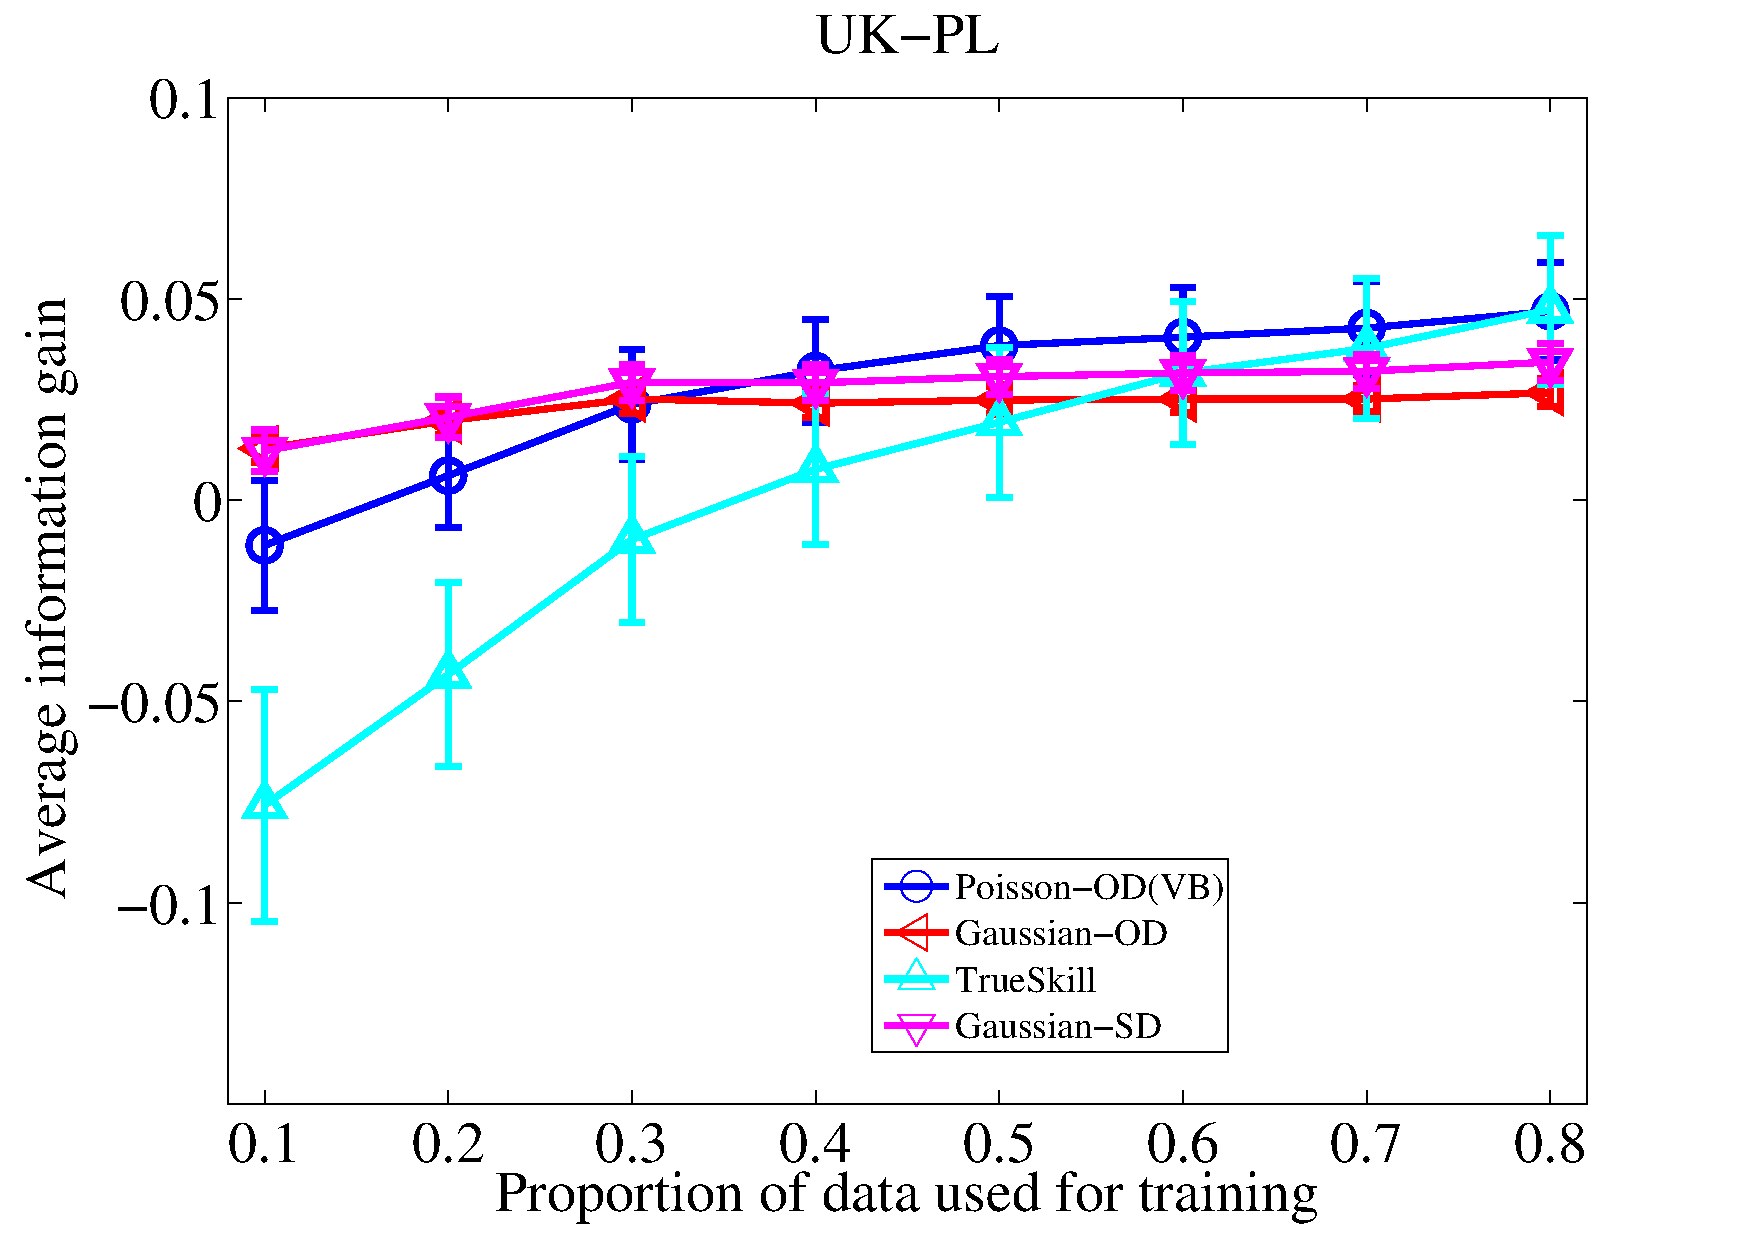
\epsfig{file=InforGain_UK, angle=0, height=8cm}
\caption{\small Results on the UK-PL, evaluated
using information gain. Error bars indicate
95\% confidence intervals.}
\label{fig:InforGain_UK}
\end{figure*}
\end{center}

Empirical evaluations with the information gain criterion on the AFL data set is shown in Figure~\ref{fig:InforGain_AFL}. We observed that all the proposed models significantly outperform TrueSkill for limited data, which further validates our hypothesis that information carried by score-based match outcomes are very helpful for skill learning when only small amount of data is available for training. When more data is available, TrueSkill improved its performance and performed the best, which indicates that updating skill levels with win/lose/draw based outcomes is more robust comparing with that based on the possibly noisy scores. 

Across the three proposed models of the AFL data set, the Poisson-OD model significantly outperforms the Gaussian models, which agrees with the fact that the exponential term in the Poisson-OD model can effectively learn relatively large match outcomes. Note that the average score for the AFL data set is 95.4 vs 1.3 for that of the UK data set. 

\begin{center}
\begin{figure*}[htbp!]
 \centering
 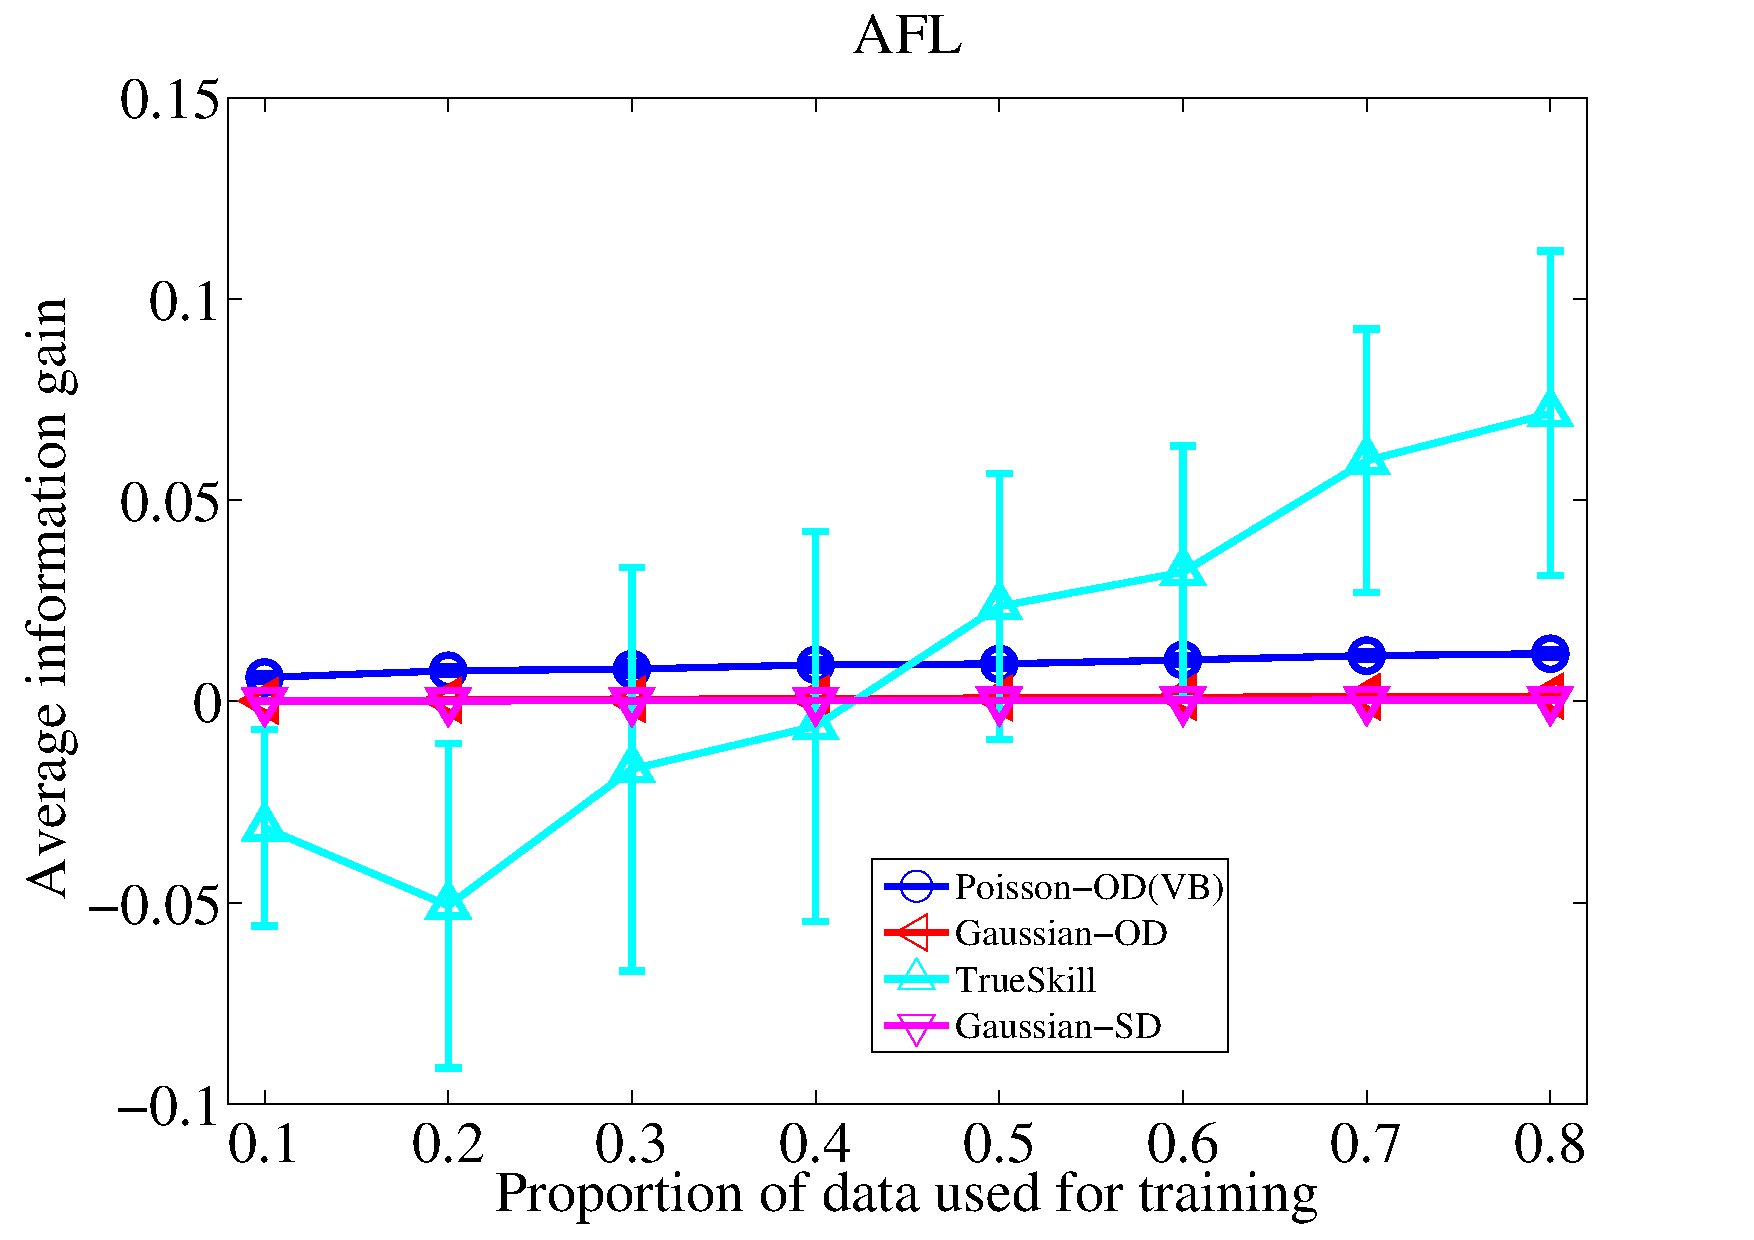
\epsfig{file=InforGain_AFL, angle=0, height=8cm}
\caption{\small Results on the AFL data set, evaluated
using information gain. Error bars indicate
95\% confidence intervals.}
\label{fig:InforGain_AFL}
\end{figure*}
\end{center}

Results on the Halo data set are shown in Figure~\ref{fig:InforGain_Halo}, and indicated that all the three proposed models significantly outperform TrueSkill for all training setting. For this data set with small average scores, the Gaussian models clearly outperform the Poisson-OD model, which further supports the fact that the amplification due to the exponential term in the Poisson-OD model may hurt the performance. For the Gaussian models, the Gaussian-OD model that separately model offence and defence skills achieves significantly better performance than the Gaussian-SD model, indicating the importance of modeling these two skill aspects separately. 

\begin{center}
\begin{figure*}[t!]
 \centering
 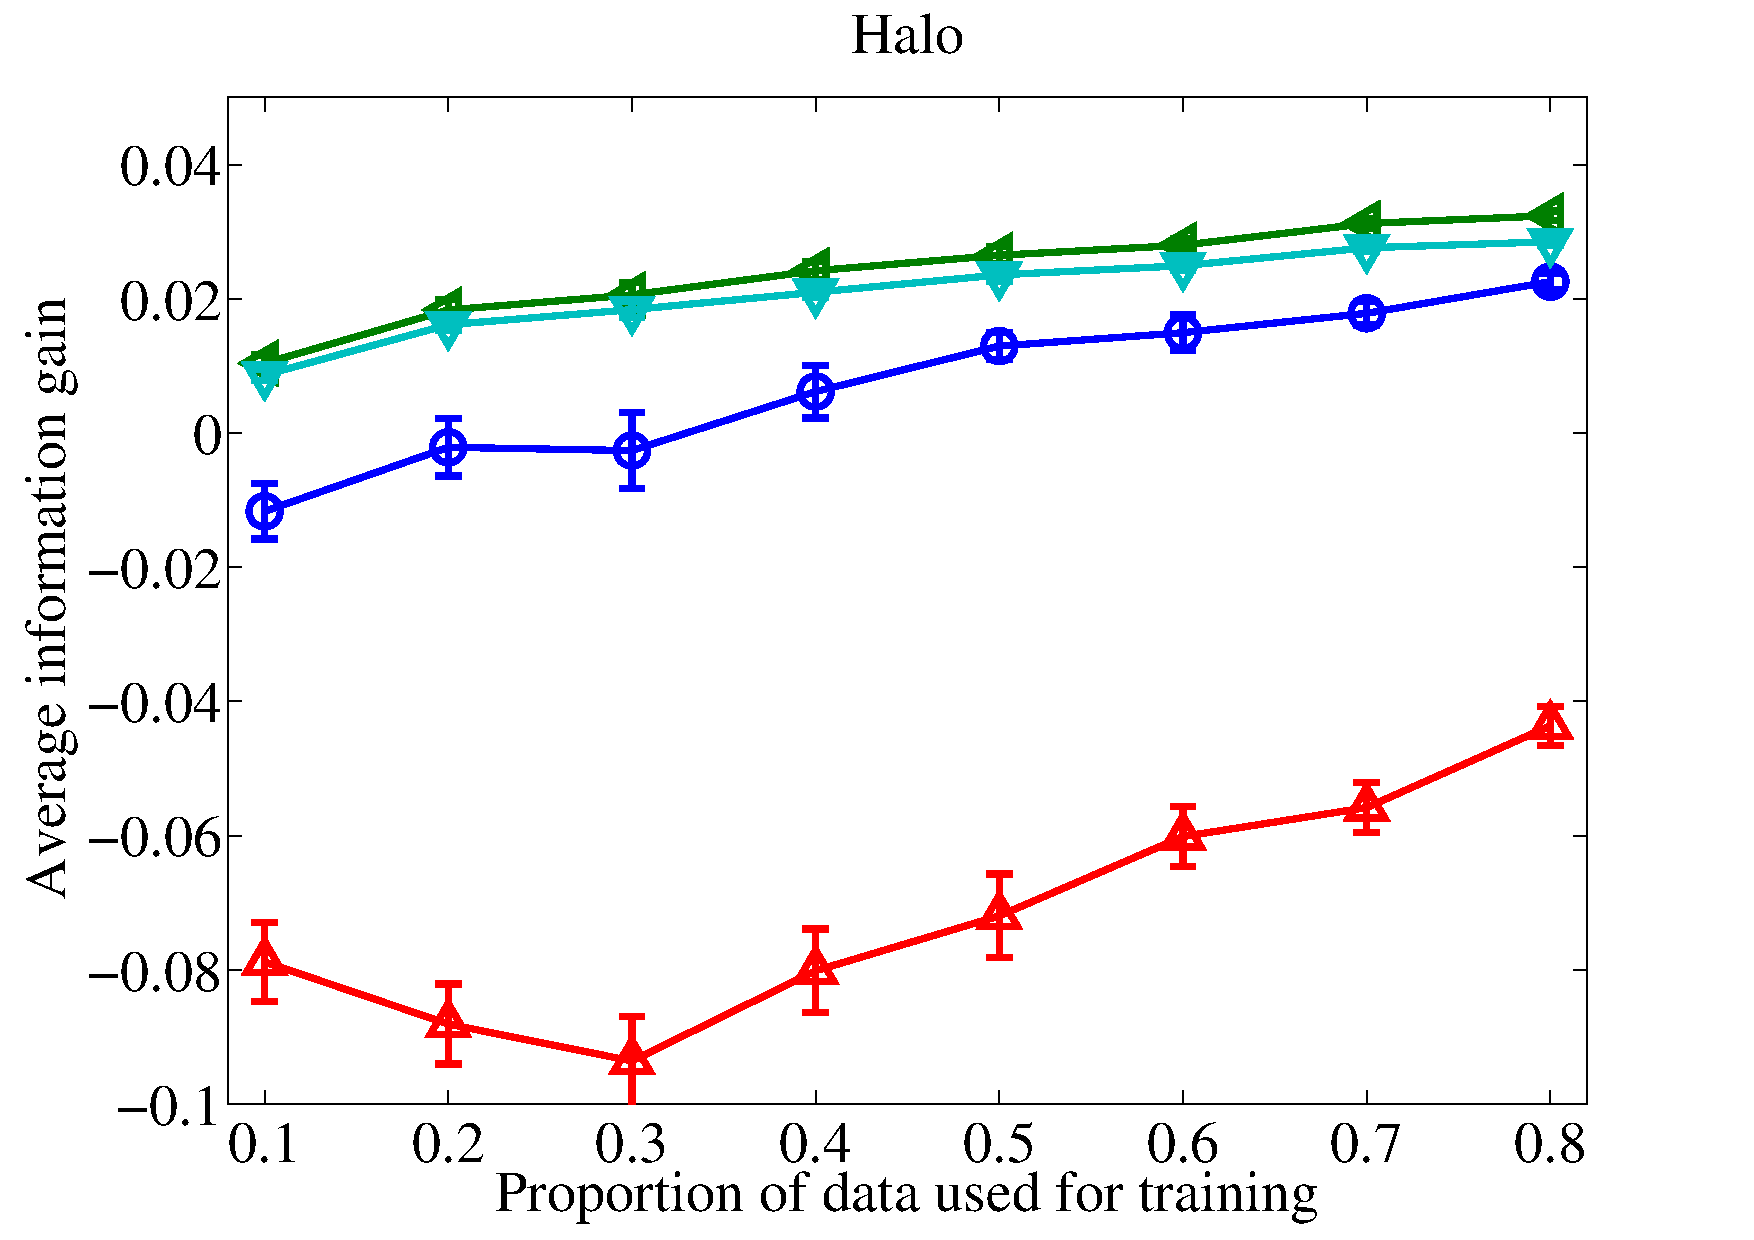
\epsfig{file=InforGain_Halo, angle=0, height=8cm}
\caption{\small Results on the Halo 2 data set, evaluated
using information gain. Error bars indicate
95\% confidence intervals.}
\label{fig:InforGain_Halo}
\end{figure*}
\end{center}

As a short summary for the results on the information gain, our observed that all the proposed models can outperform the TrueSkill for most of the training settings, and the differences are significant particularly for limited training data. This observation reflects our motivation of modeling the more informative score-based match outcomes in improving skill modeling. The Gaussian-OD model performs better than the Gaussian-SD model for most of the training cases, and the improvement is significant for the Halo data set, indicating the benefits of modeling the offence and defence of a team's skills. While the Gaussian models are more appropriate for the data sets with small average match scores, the Poisson model edges out for the data set with large score match outcomes. 

\subsubsection{Win/no-Win Prediction Accuracy }

In terms of win/no-win prediction accuracy, the Gaussian-OD model generally
provides the best average AUC, followed by Gaussian-SD, then
TrueSkill, then Poisson-OD model for both the UK and AFL data set corresponding to Figure~\ref{fig:WLAccuracy_UK} and Figure~\ref{fig:WLAccuracy_AFL}. The better performance by the Gaussian-OD model indicated the benefits of separating offence/defence skill modeling in the Gaussian-OD model, achieving a performance edge over the combined skill model of the Gaussian-SD model.

\begin{center}
\begin{figure*}[htbp!]
 \centering
 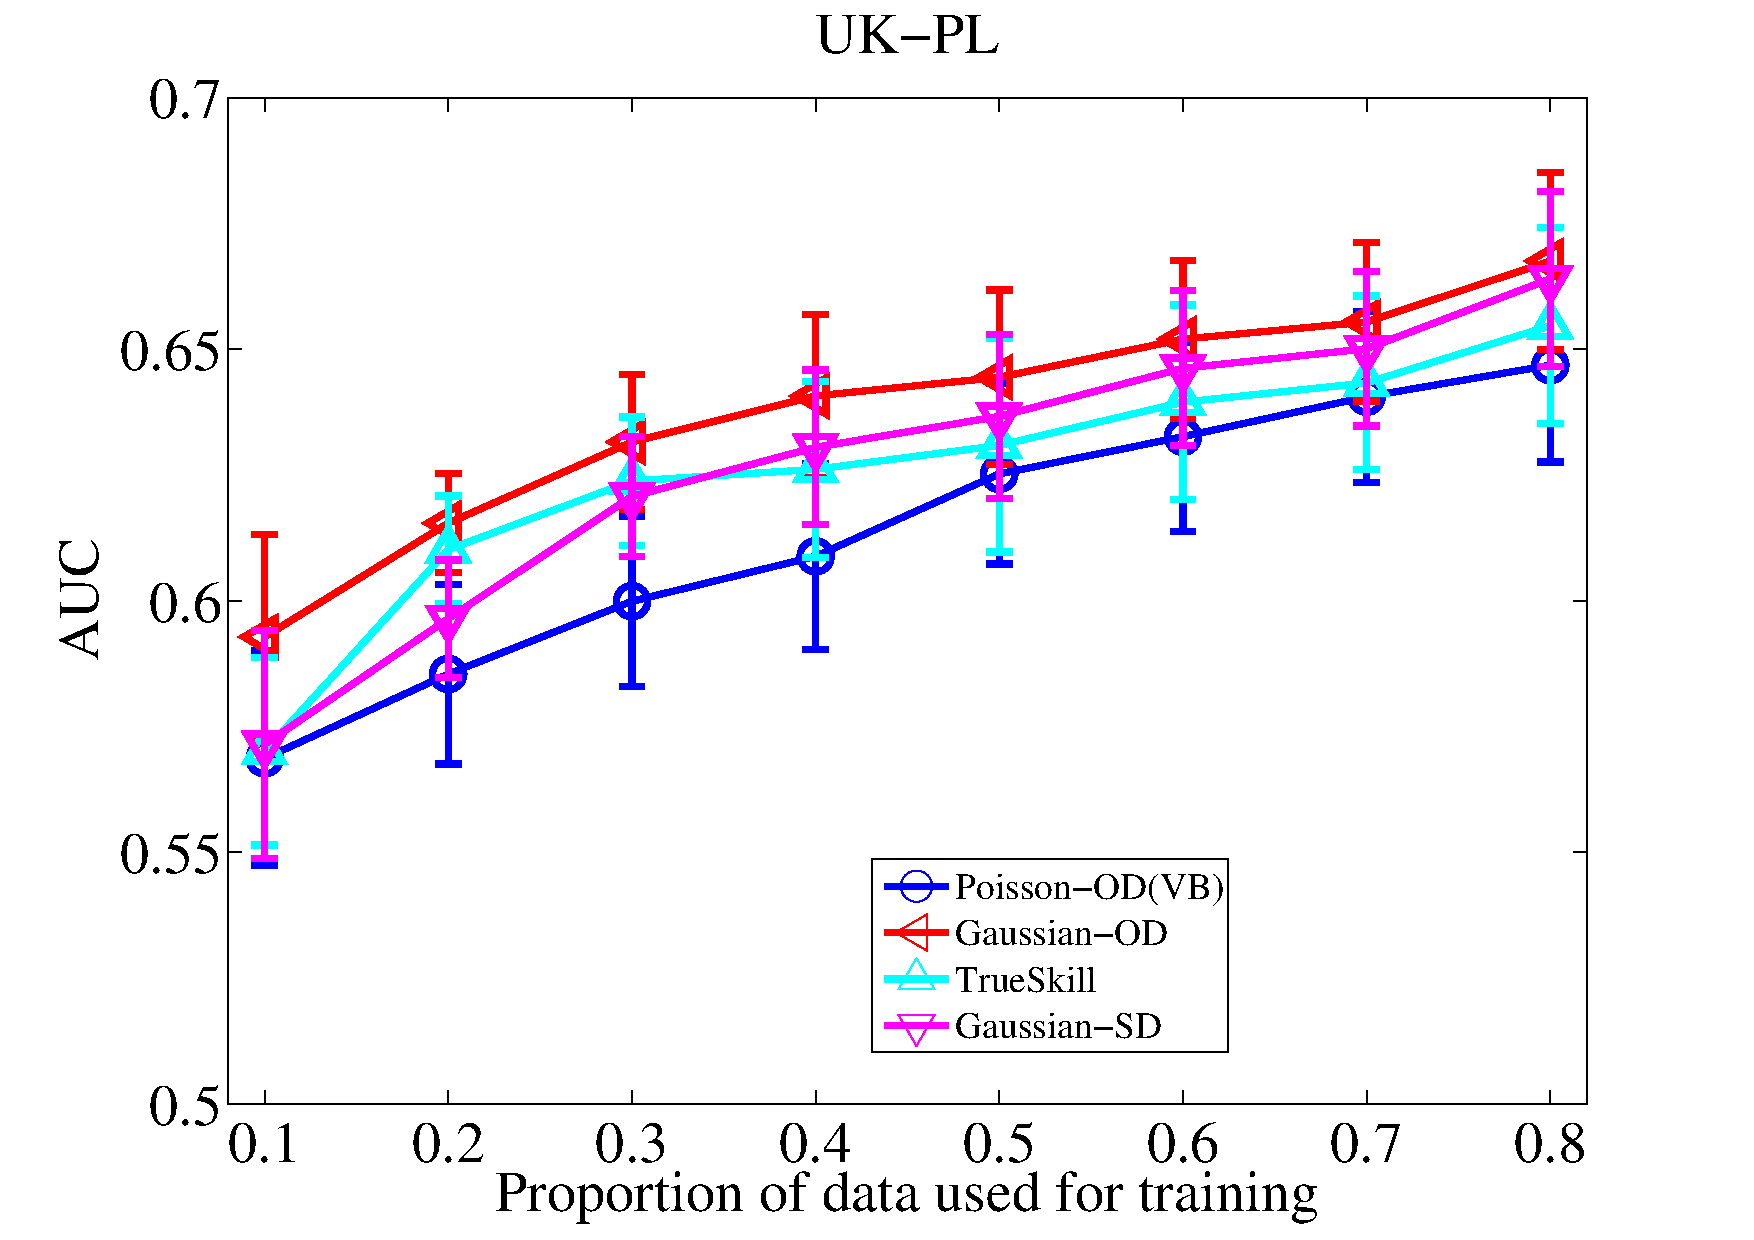
\epsfig{file=WLAccuracy_UK, angle=0, height=8cm}
\caption{\small Results on the UK-PL, evaluated using win/loss prediction accuracy in
term of the area of the curve (AUC). Error bars indicate
standard errors.}
\label{fig:WLAccuracy_UK}
\end{figure*}
\end{center}


\begin{center}
\begin{figure*}[htbp!]
 \centering
 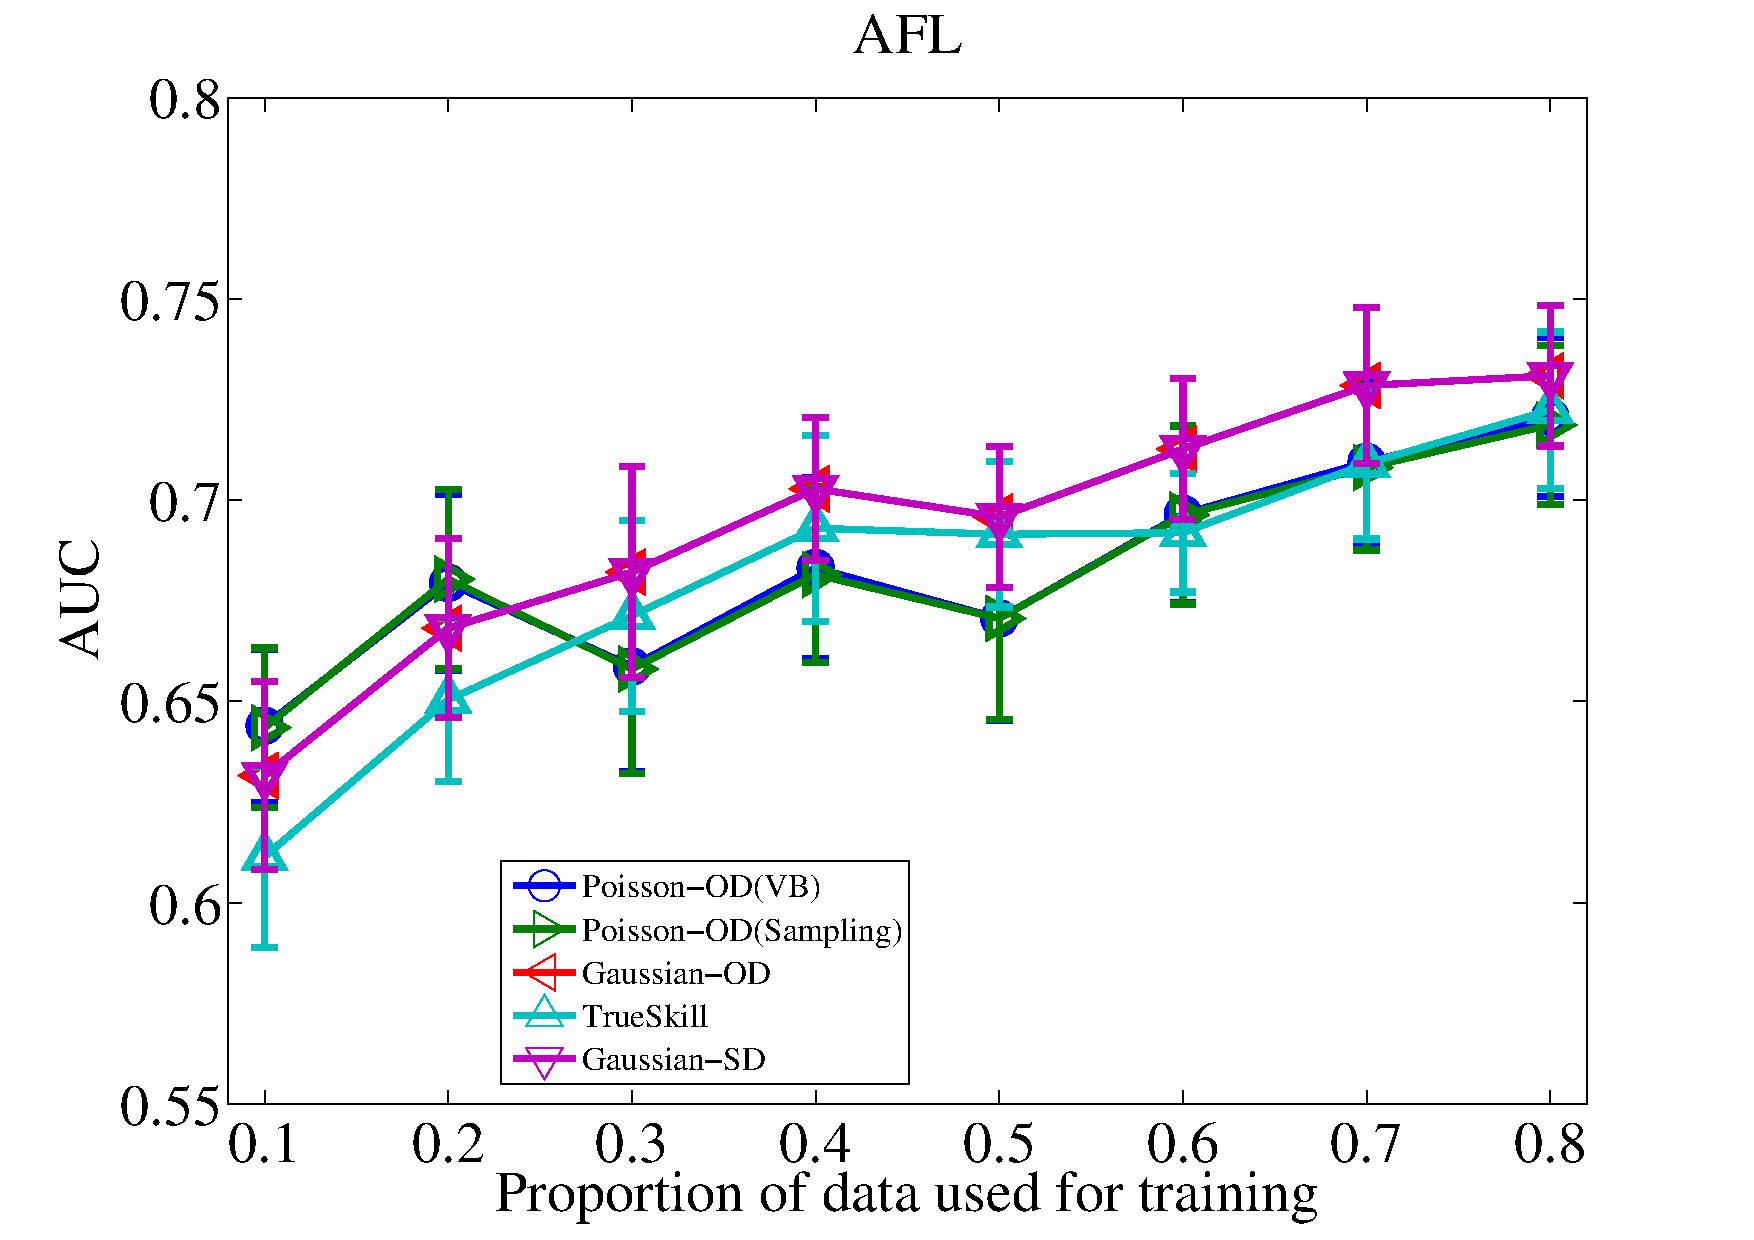
\epsfig{file=WLAccuracy_AFL, angle=0, height=8cm}
\caption{\small Results on the AFL data set, evaluated using win/loss prediction accuracy in
term of the area of the curve (AUC). Error bars indicate
standard errors.}
\label{fig:WLAccuracy_AFL}
\end{figure*}
\end{center}

\begin{center}
\begin{figure*}[htbp!]
 \centering
 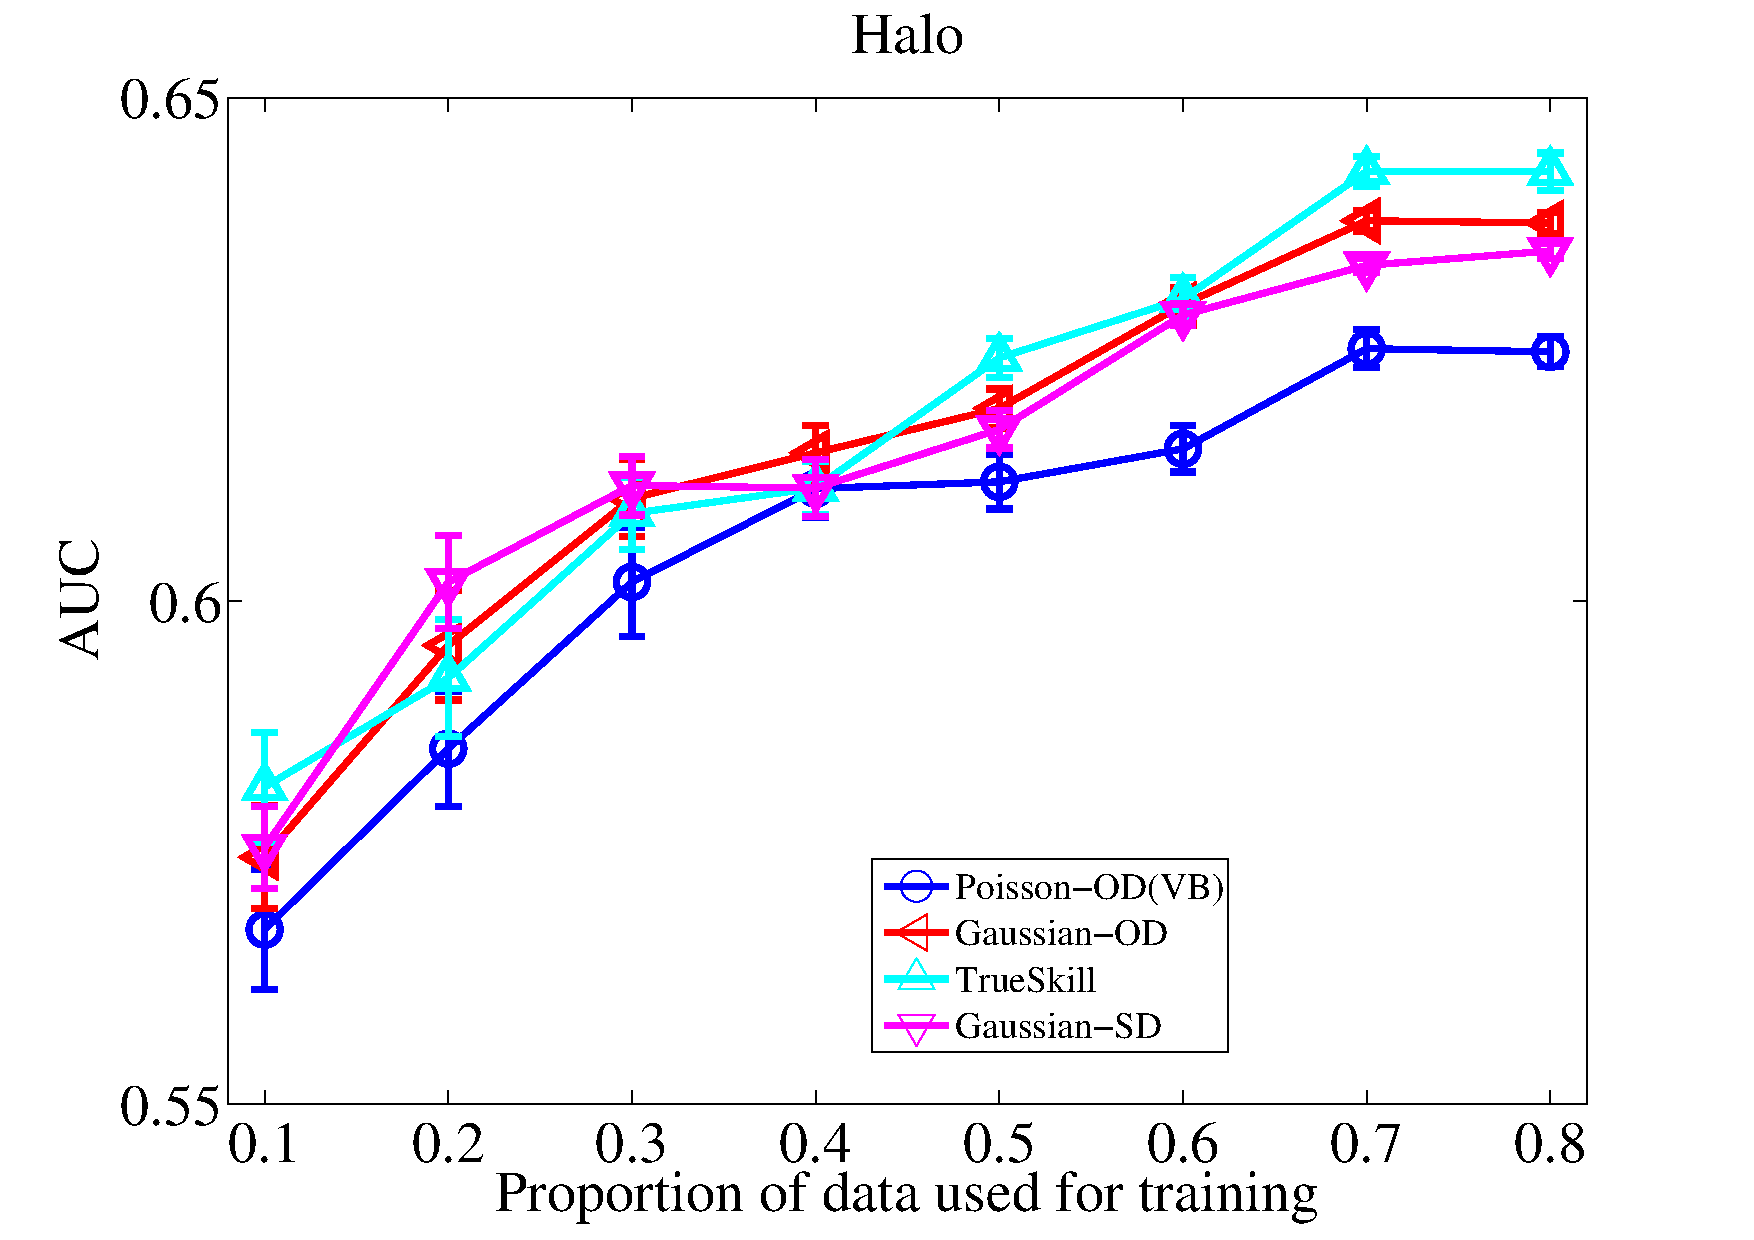
\epsfig{file=WLAccuracy_Halo, angle=0, height=8cm}
\caption{\small Results on the Halo 2 data set, evaluated using win/loss prediction accuracy in
term of the area of the curve (AUC). Error bars indicate
standard errors.}
\label{fig:WLAccuracy_Halo}
\end{figure*}
\end{center}
%We check the statistics of the match outcomes
%(Table~\ref{table:datasetStatistics}),
%and observe that the average
%scores for the UK-PL, Halo, and AFL datasets are 1.3, 42.7, and 95.4,
%respectively.  From this, we might infer the Poisson-OD model predicts better
%when the average scores for a dataset are relatively larger numbers;
%here it seems the exponential term used in the Poisson model can help
%amplify small performance differences to explain high scores, leading
%to more stable skill modeling in high-scoring games.

\subsubsection{Win/Lose/Draw Prediction with Brier Score}
We further studied the performances of various models with the Brier Score in a multi-class classification setting, where each game is an observation and the class for the observation between two teams $(i, j)$ is in $\{i\text{ win}, i\text{ lose}, \text{ draw}\}$. Comparing with the previous reported performance on Win/no-Win, the Brier score we used for multi-class classification can handle the matches that are a draw between the participating teams. 

For the results on the UK and AFL data set shown in Figure~\ref{fig:WLAccuracy_UK_BrierScore} and Figure~\ref{fig:WLAccuracy_AFL_BrierScore}, we observed that the the standard errors for all the models are much larger, indicating that the performance differences between these models are not significant. For the Brier score of UK-PL data set (Figure~\ref{fig:WLAccuracy_UK_BrierScore}), the Poisson-OD and the Gaussian models seem to outperform TrueSkill for limited training data. Within the three proposed model, the Gaussian models slightly edge out the Poisson-OD model, which is again due to the scores for the UK data set are relatively small numbers. 
\begin{center}
\begin{figure*}[t!]
 \centering
 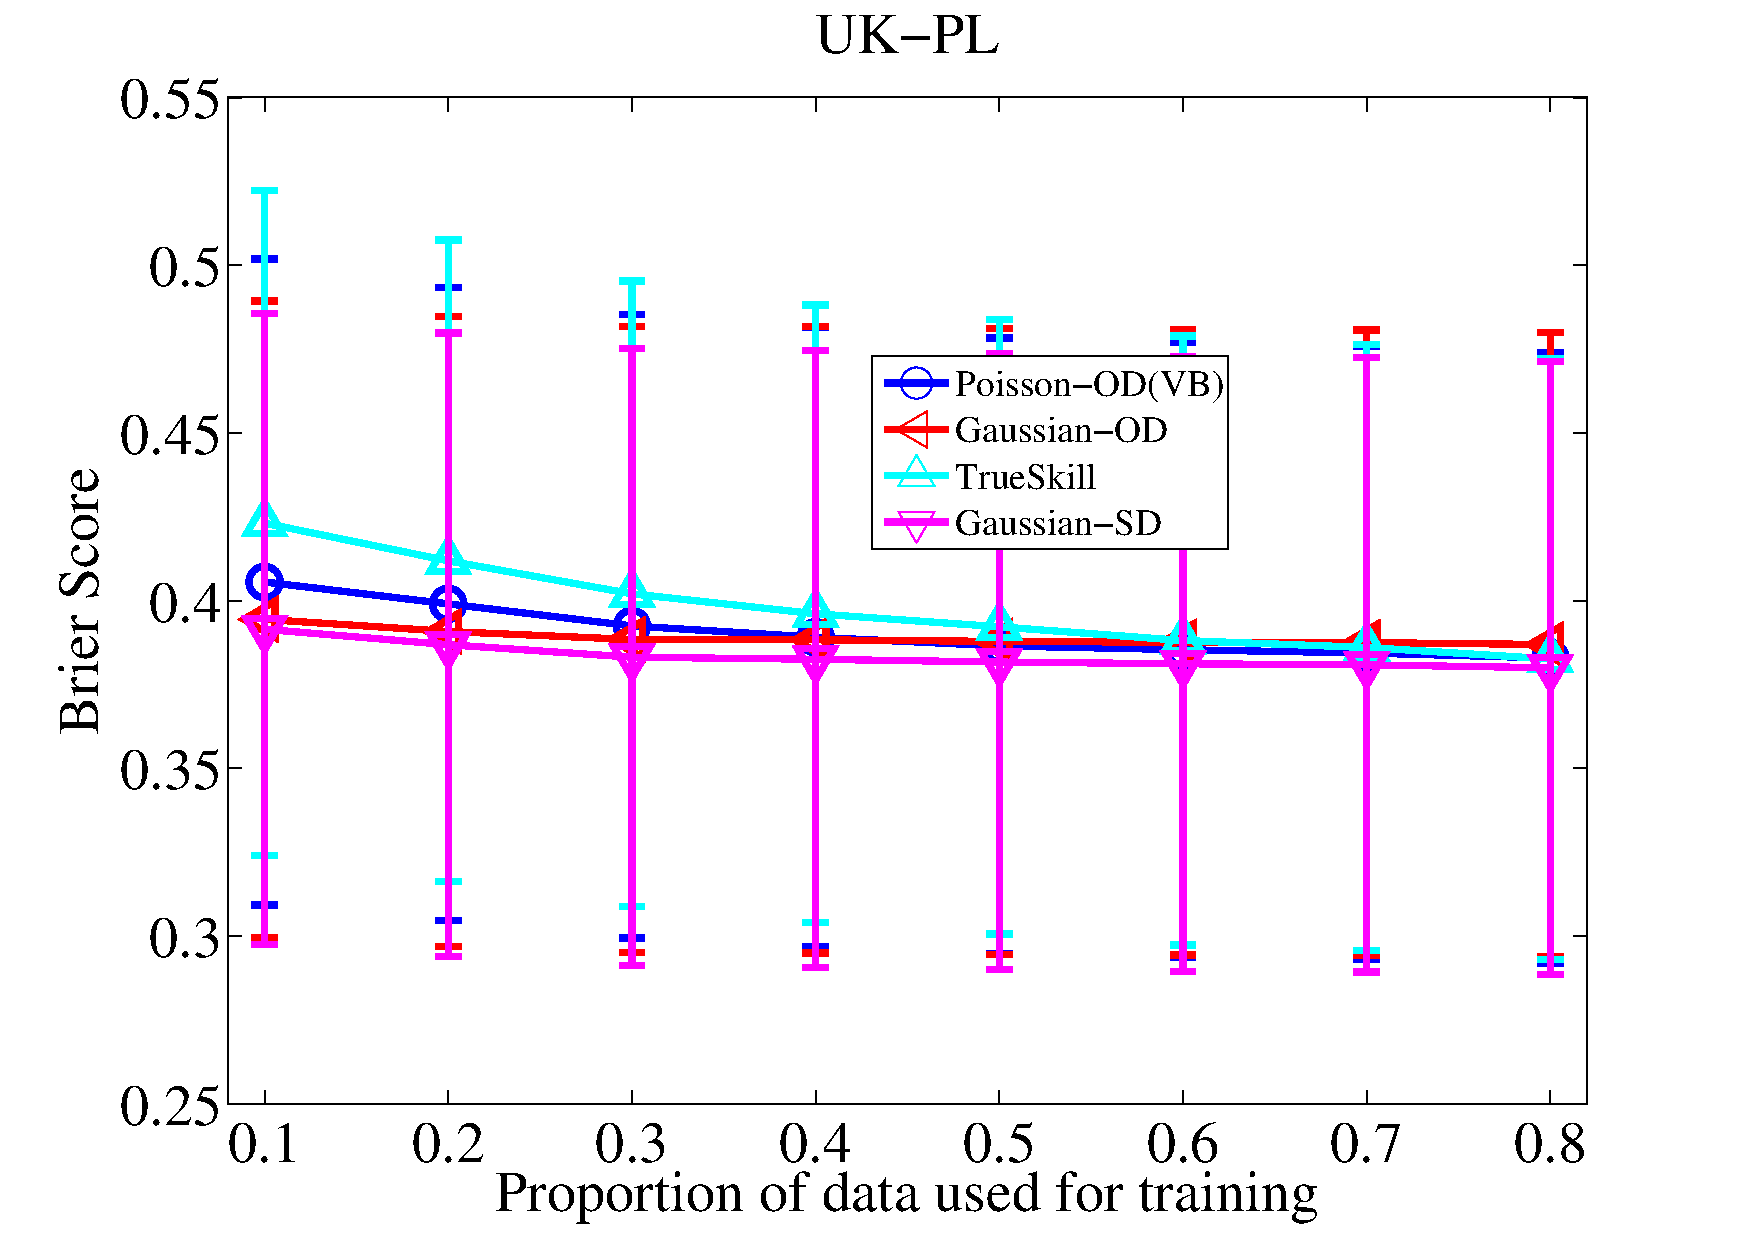
\epsfig{file=WLAccuracy_UK_BrierScore, angle=0, height=8cm}
\caption{\small Results on the UK data set, evaluated using the Brier Score for multi-class classification. Error bars indicate
standard errors.}
\label{fig:WLAccuracy_UK_BrierScore}
\end{figure*}
\end{center}

For the AFL data set (Figure~\ref{fig:WLAccuracy_AFL_BrierScore}), results indicated that the proposed models perform much better than the TrueSkill, although TrueSkill reached the best possible performance of the Poisson-OD, Gaussian-OD, and Gaussian-SD when sufficiently large amount of data is used for training. Across the three proposed models, the Poisson-OD model slightly outperform the Gaussian models, however the performance difference is not significant. 
\begin{center}
\begin{figure*}[t!]
 \centering
 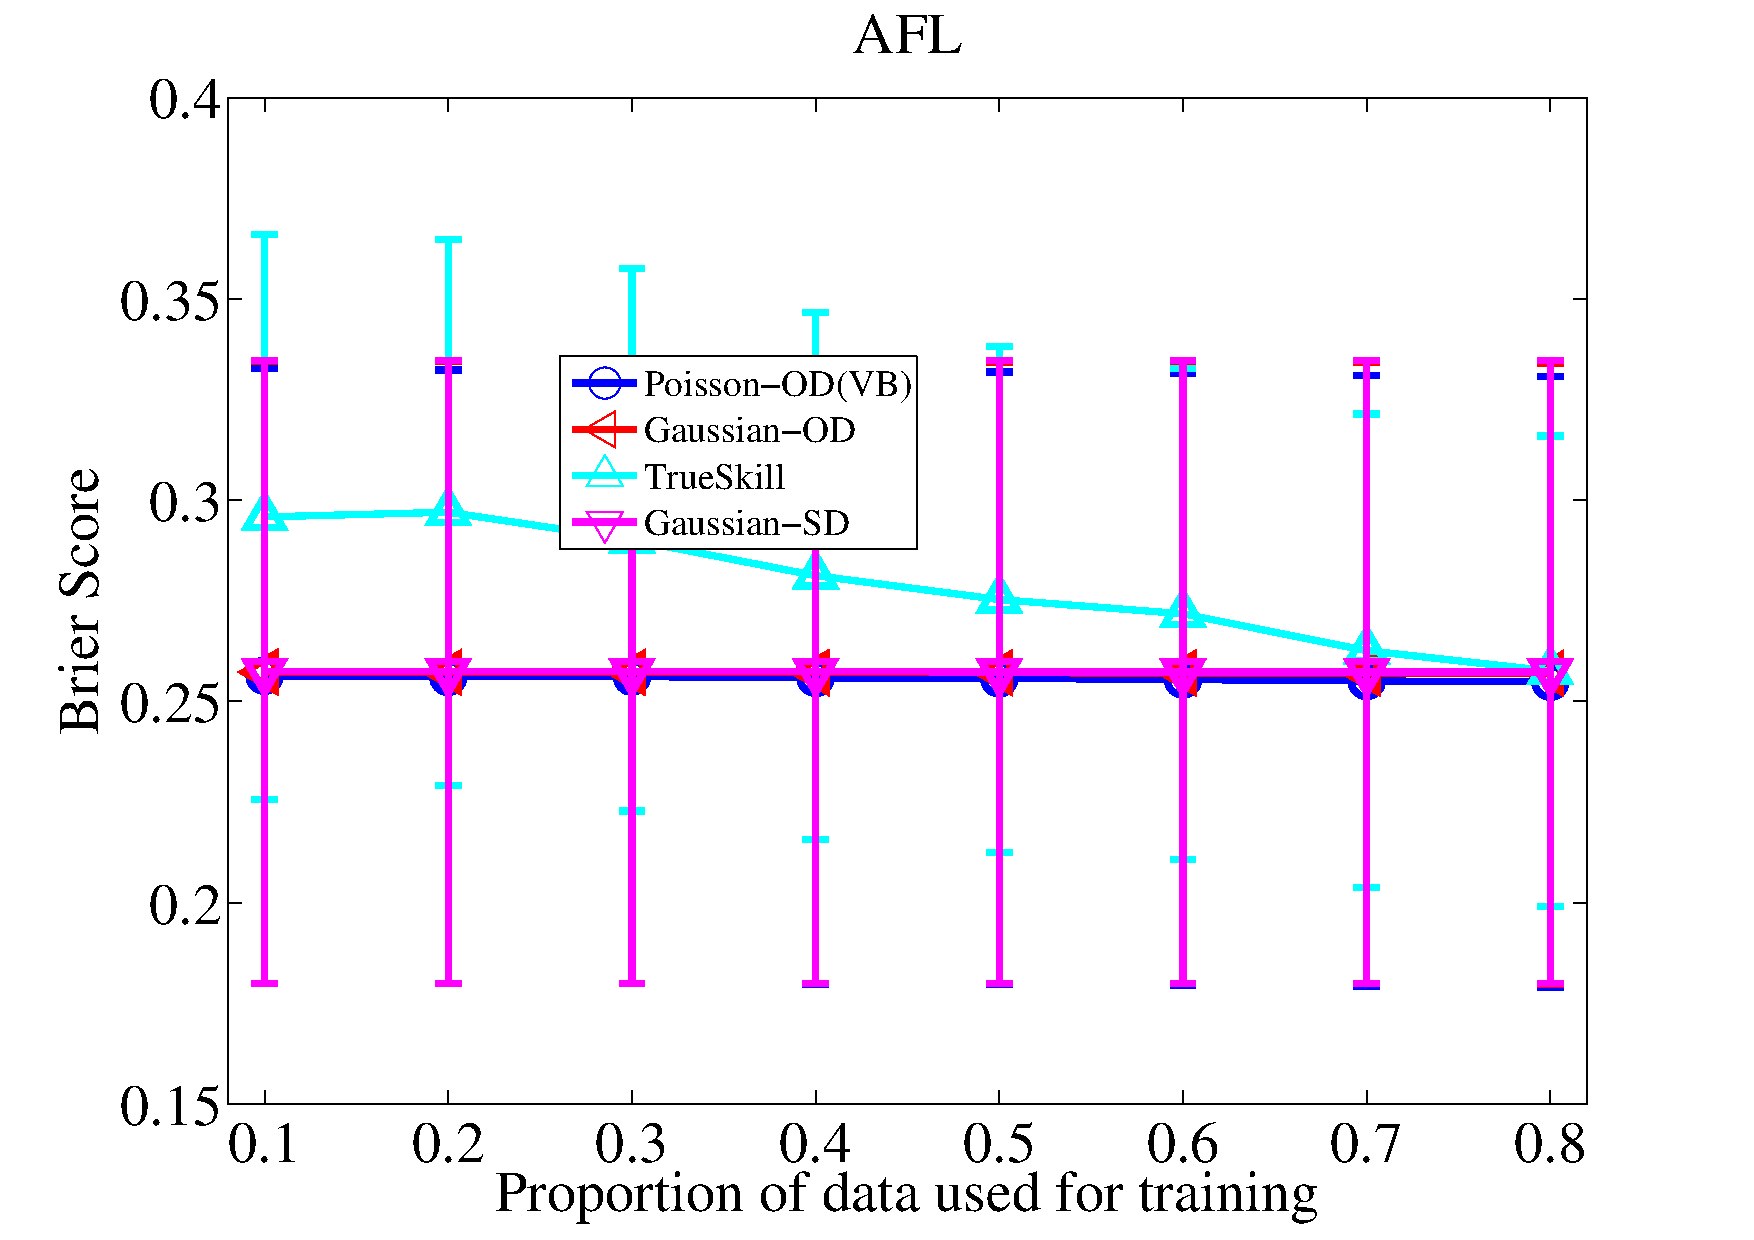
\epsfig{file=WLAccuracy_AFL_BrierScore, angle=0, height=8cm}
\caption{\small Results on the AFL data set, evaluated using the Brier Score for Win/Lose/Draw prediction. Error bars indicate
standard errors.}
\label{fig:WLAccuracy_AFL_BrierScore}
\end{figure*}
\end{center}

\begin{center}
\begin{figure*}[t!]
 \centering
 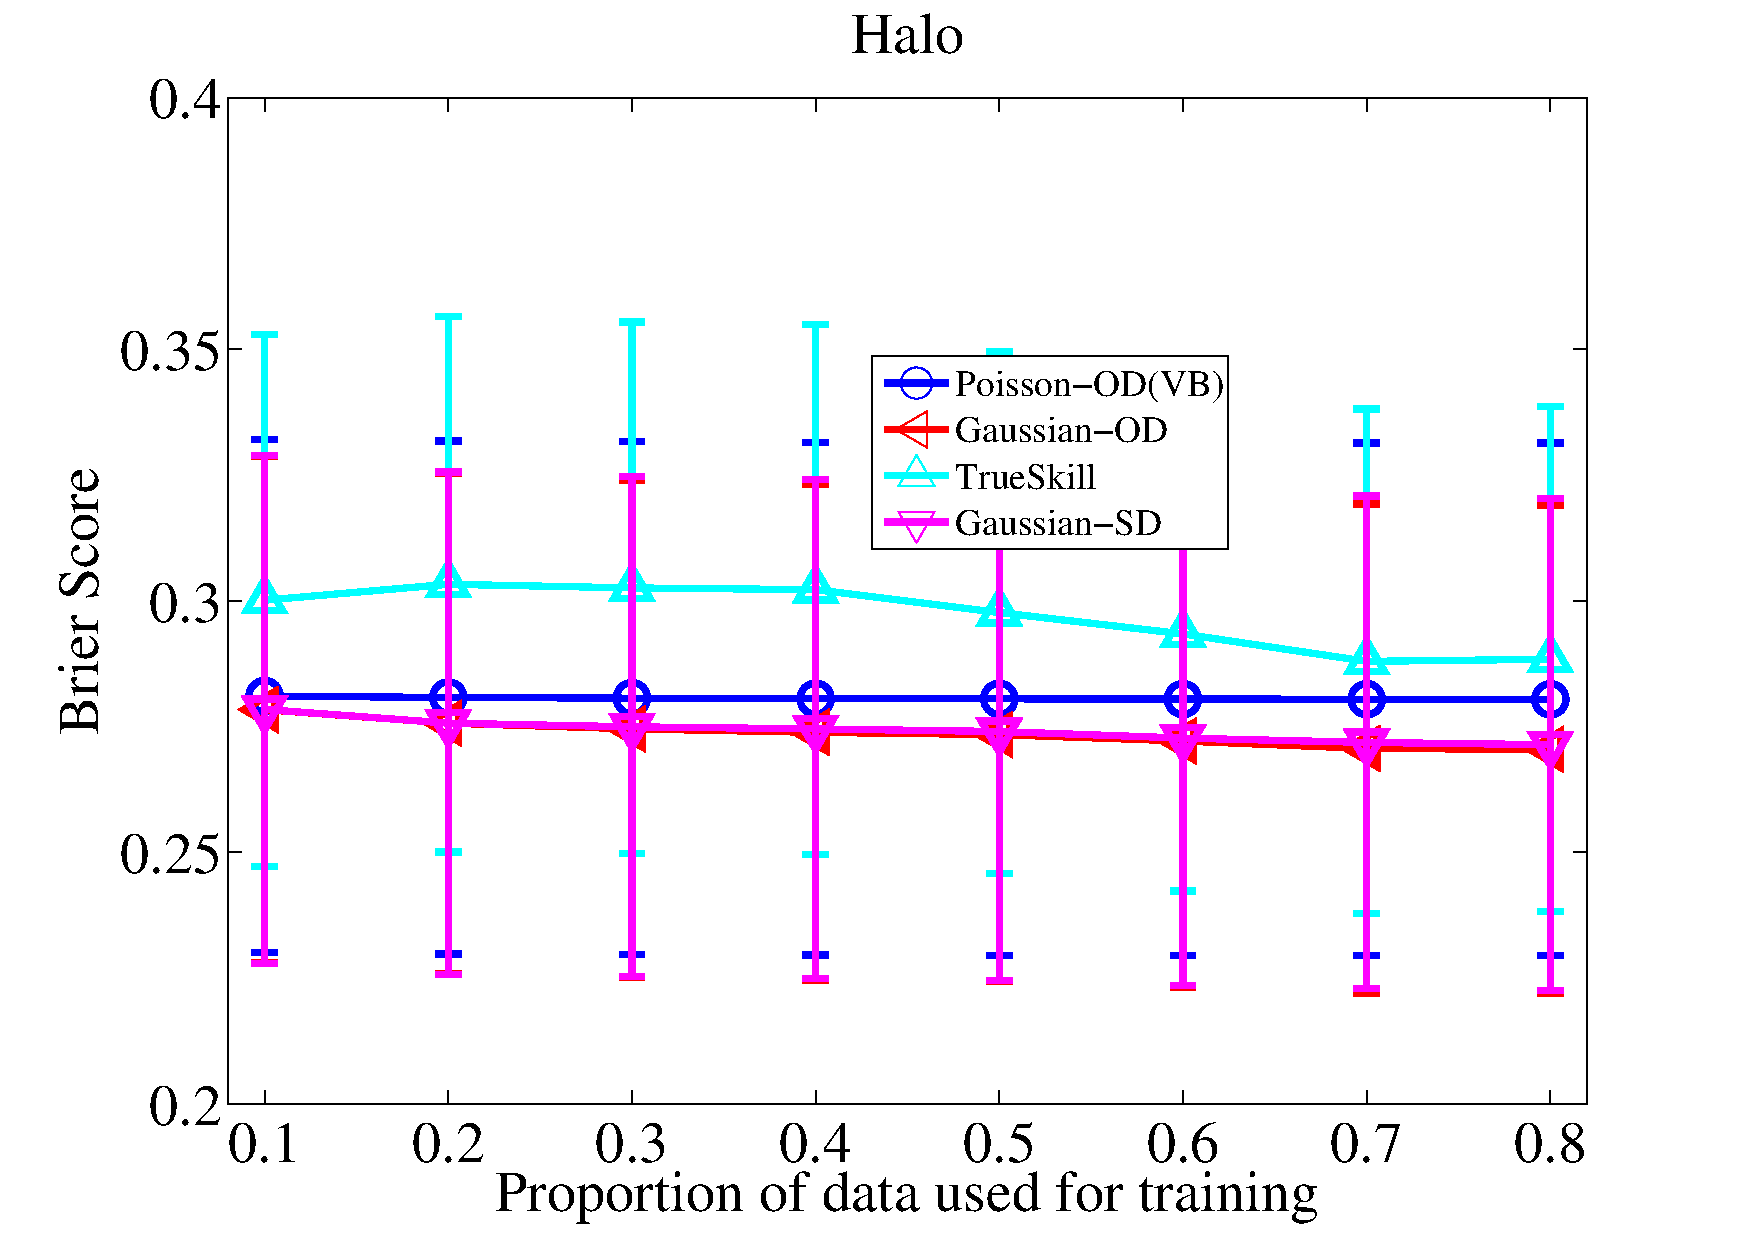
\epsfig{file=WLAccuracy_Halo_BrierScore, angle=0, height=8cm}
\caption{\small Results on the Halo data set, evaluated using the Brier Score for Win/Lose/Draw prediction. Error bars indicate
standard errors.}
\label{fig:WLAccuracy_Halo_BrierScore}
\end{figure*}
\end{center}

When comparing the best performance on the AFL and UK dataset, we note that the Brier Score is much lower for the AFL data set (close to 0.25) comparing with the UK data set (close to 0.38), indicating that predicting the football games may be much harder than that the rugby games. 


\subsubsection{Score Prediction Errors}
%\paragraph{Score Prediction Errors}

%For the Gaussian-SD model, we note that the average relative score
%difference error is close 1 indicating the predicted difference is
%probably close to 0 with it being on the correct side of 0 as more
%training data is used.
%The Gaussian-OD model predicts more accurate scores on the UK-PL and
%Halo datasets, and Poisson-OD is more accurate for the AFL dataset.
%This can be explained by a simple skill analysis --- the learned
%skills on the UK-PL dataset tend to show a larger variance (for all
%models), whereas the learned skills on the AFL dataset show little
%variance (for all models except Gaussian-SD).  To confirm our
%previous hypothesis, the use of an exponentiated scoring rate in the
%Poisson model allows it to amplify small performance differences in
%the learned AFL skills to make more accurate score predictions on AFL
%data.  This amplification appears to hurt the Poisson-OD model on the
%relative low-scoring UK-PL dataset.

We report the score prediction errors for different data sets in Figure~\ref{fig:ScoreError_AFL}, Figure~\ref{fig:ScoreError_UK}, and Figure~\ref{fig:ScoreError_Halo}. Gaussian-OD predicts more accurate scores on the UK-PL, while Poisson-OD is more accurate for the AFL dataset. For the AFL data set (Figure~\ref{fig:ScoreError_AFL}), we observed that the Gaussian-OD model clearly failed in predicting the scores of the matches, because the differences in the learned skill levels between teams are relatively small. A Gaussian likelihood function with the small difference has low probability of generating huge match scores for the AFL data set. Given the same difference, the Poisson-OD model with an exponentiated scoring rate would seem to amplify these small performance differences in learned AFL skills to make more accurate score predictions on AFL data.  This amplification appears to hurt the Poisson-OD model on the lower-scoring UK-PL (the mean score for the AFL data is 95.4 vs 42.7 and 1.3 respectively for the Halo 2 and UK-PL data).

\begin{center}
\begin{figure*}[htbp!]
 \centering
 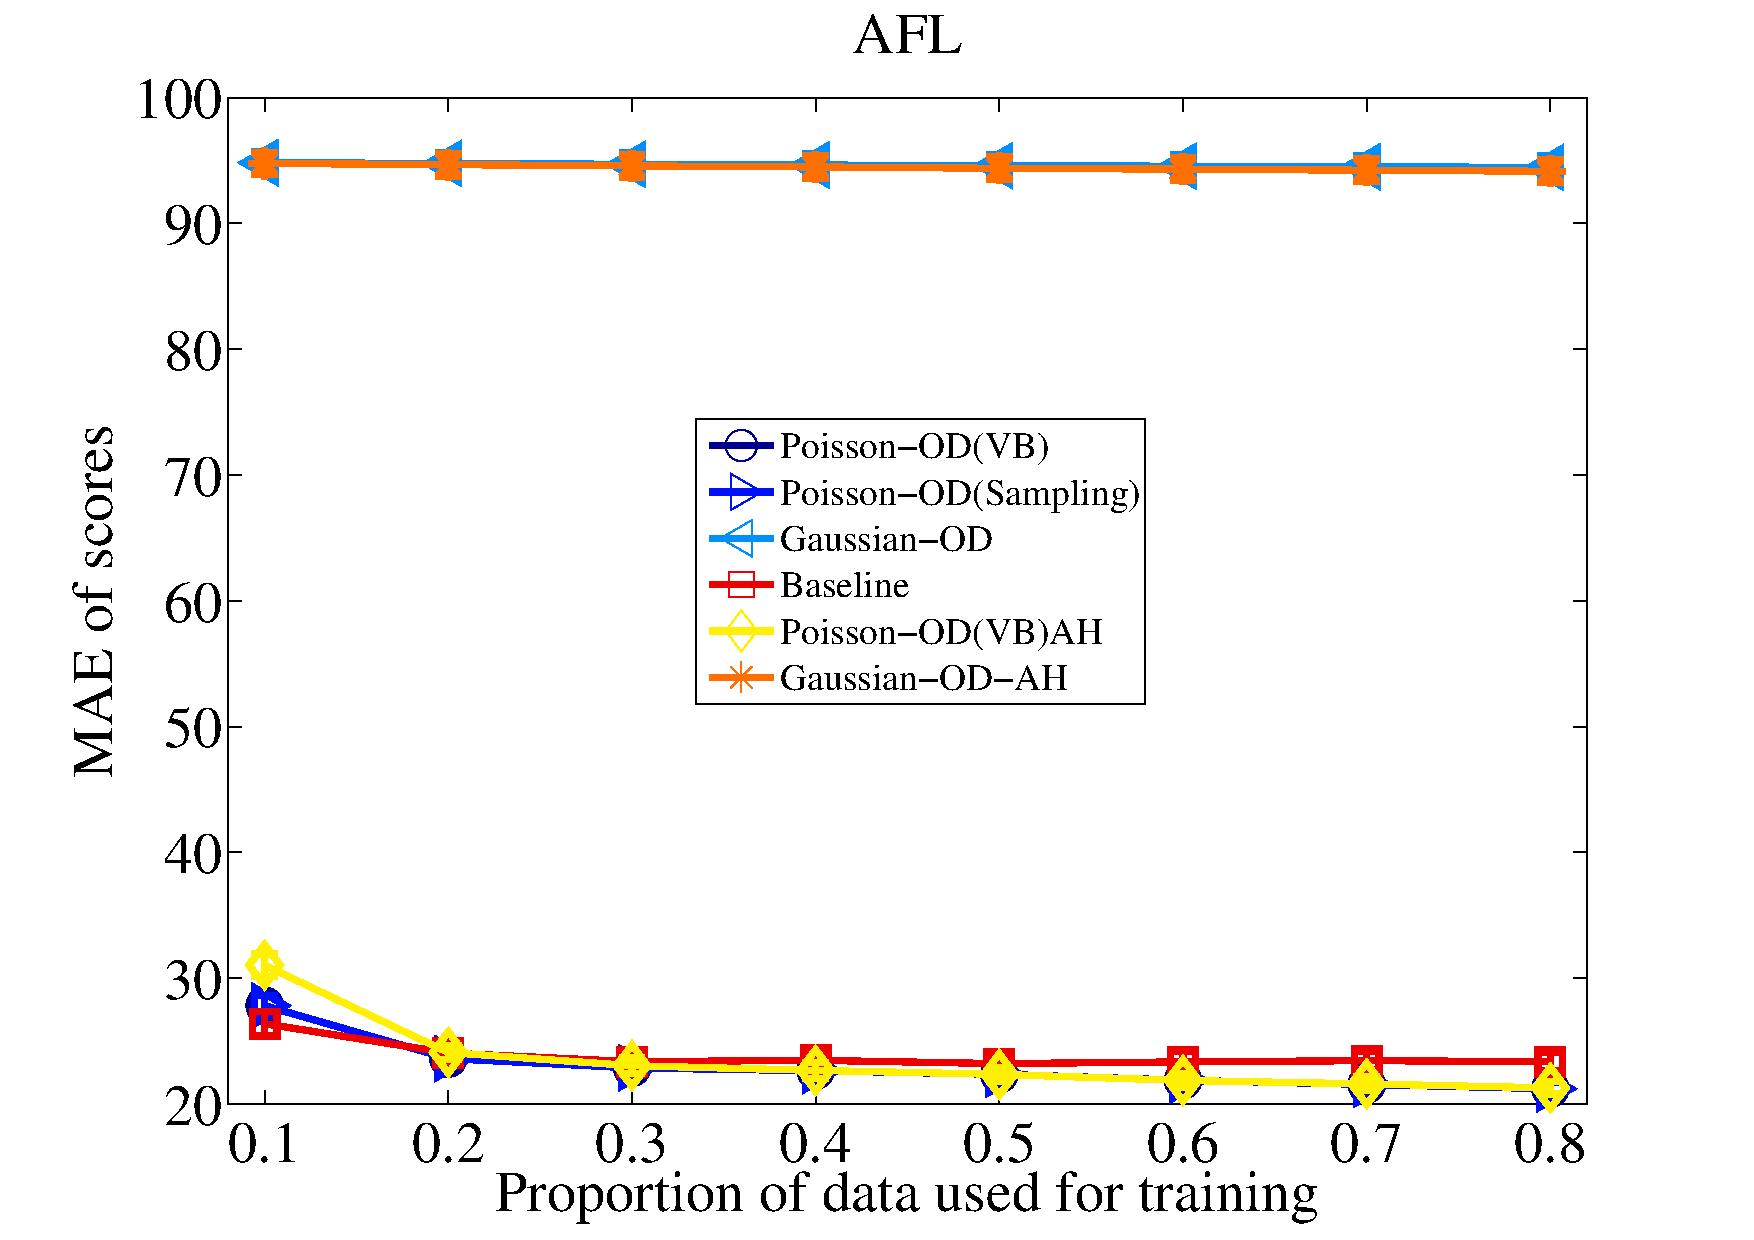
\epsfig{file=ScoreError_AFL, angle=0, height=8cm}
\caption{\small Results on the AFL data set, evaluated using win/loss prediction accuracy in
term of the area of the curve (AUC). Error bars indicate
standard errors.}
\label{fig:ScoreError_AFL}
\end{figure*}
\end{center}

As inclusion of the Gaussian-OD model makes the comparison between the Poisson model and the baseline hard to visualize, we removed the Gaussian-OD model in Figure~\ref{fig:ScoreError_AFL_without_GaussianOD} for better comparing the Poisson model and the baseline method. Interestingly, we observe that the baseline method based on average scores of each team makes better predictions than the Poisson model when only 10\% of data is used for training. This is not surprising because the belief associated with the Poisson-OD model on team skills exhibits large uncertainty when only a few observations are used for training. As we can see when more data is used for training, the Poisson-OD model performs significantly better than the baseline. Note that for the Poisson-OD model, we observed that the performances are comparable when Bayes inference is conducted by variational Bayes and slice sampling.
 
\begin{center}
\begin{figure*}[htbp!]
 \centering
 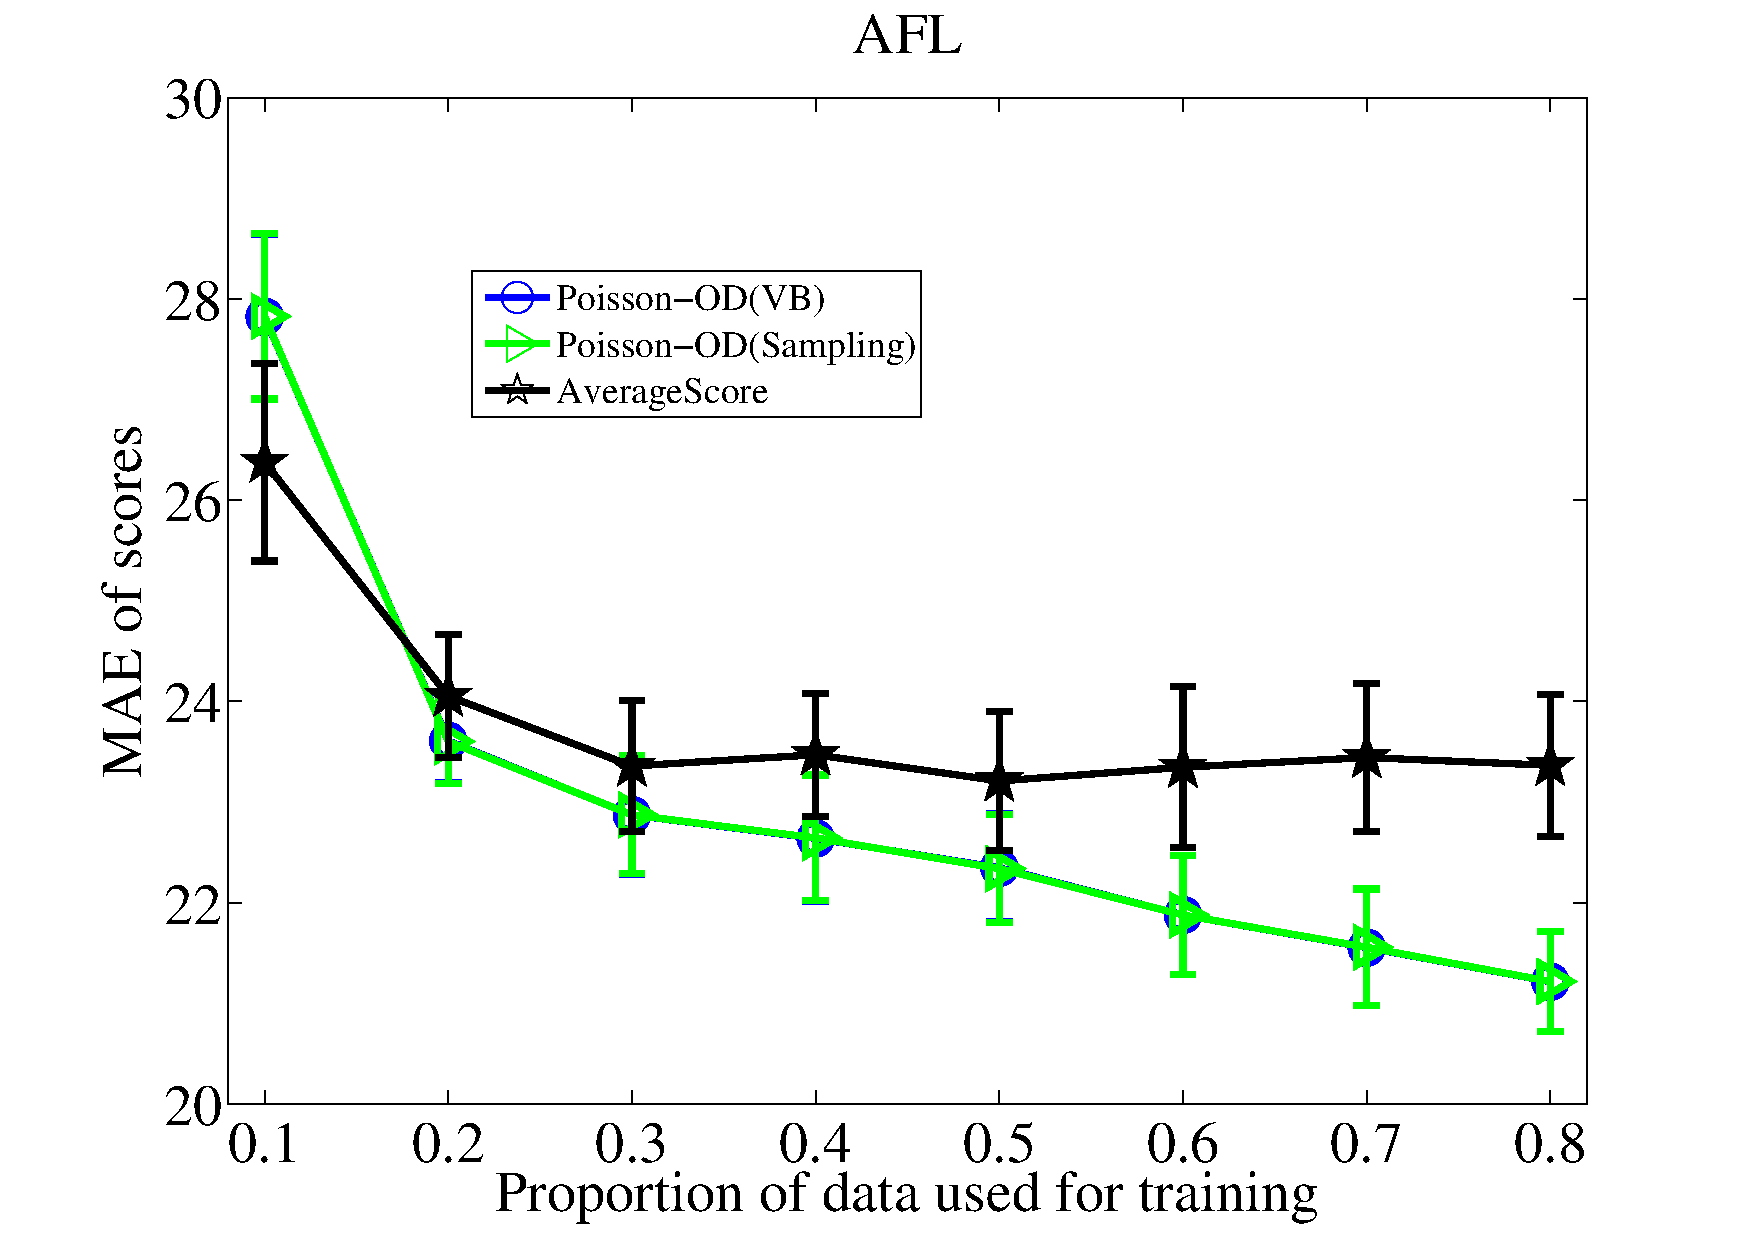
\epsfig{file=ScoreError_AFL_without_GaussianOD, angle=0, height=8cm}
\caption{\small Results on the AFL data set, evaluated using win/loss prediction accuracy in
term of the area of the curve (AUC). Error bars indicate
standard errors.}
\label{fig:ScoreError_AFL_without_GaussianOD}
\end{figure*}
\end{center}

As mentioned above for predicting scores on the UK data set (Figure~\ref{fig:ScoreError_UK}), the Poisson-OD model clearly fails in predicting this type of matches with low match scores (average scores being 1.3 for the UK data set). Given such low score matches, our Gaussian-OD models significantly outperforms the baseline for all the training settings. Our empirical results thus suggest that one can choose the models proposed in the present paper depending on the specific applications in order to achieve satisfactory results. 
\begin{center}
\begin{figure*}[t!]
 \centering
 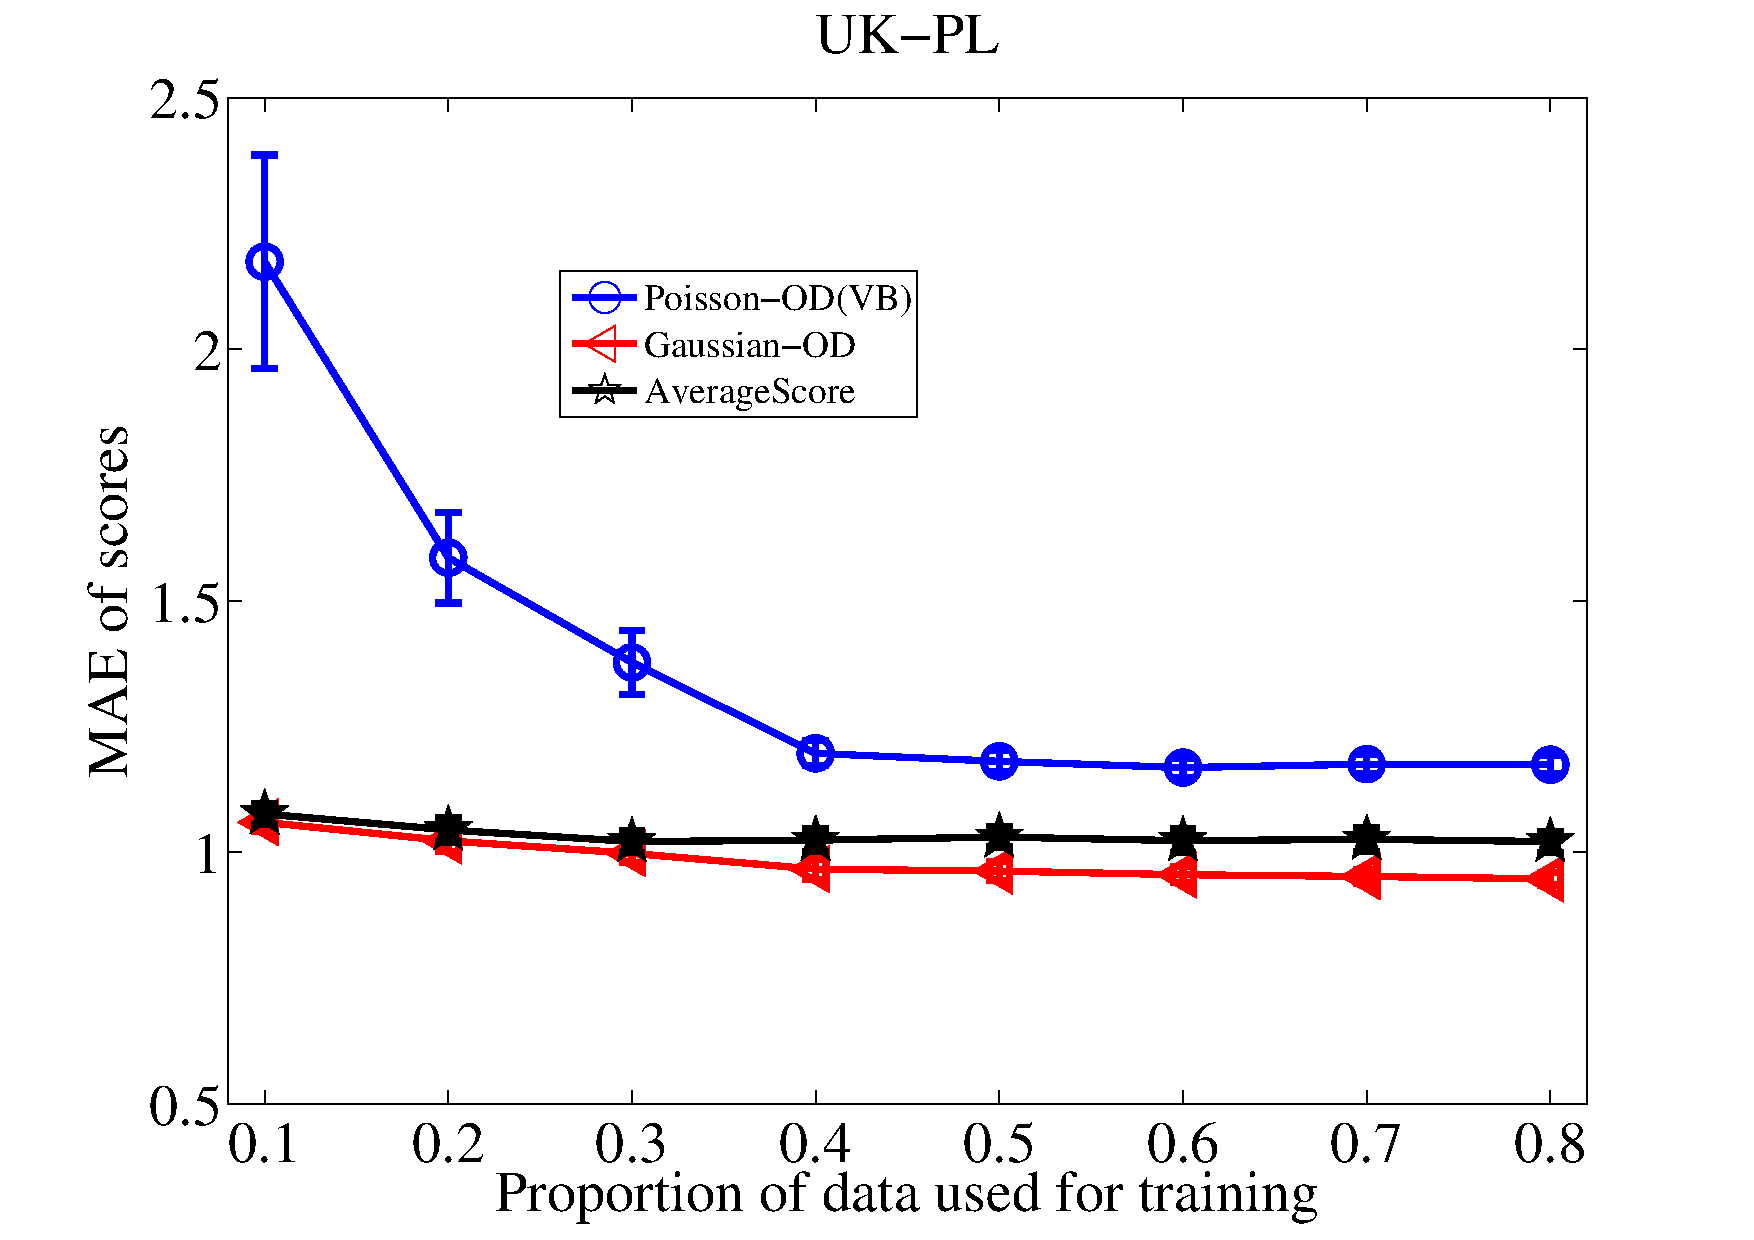
\epsfig{file=ScoreError_UK, angle=0, height=8cm}
\caption{\small Results on the UK-PL, evaluated using score
prediction error (right column). Error bars indicate
standard errors.}
\label{fig:ScoreError_UK}
\end{figure*}
\end{center}

\begin{center}
\begin{figure*}[t!]
 \centering
 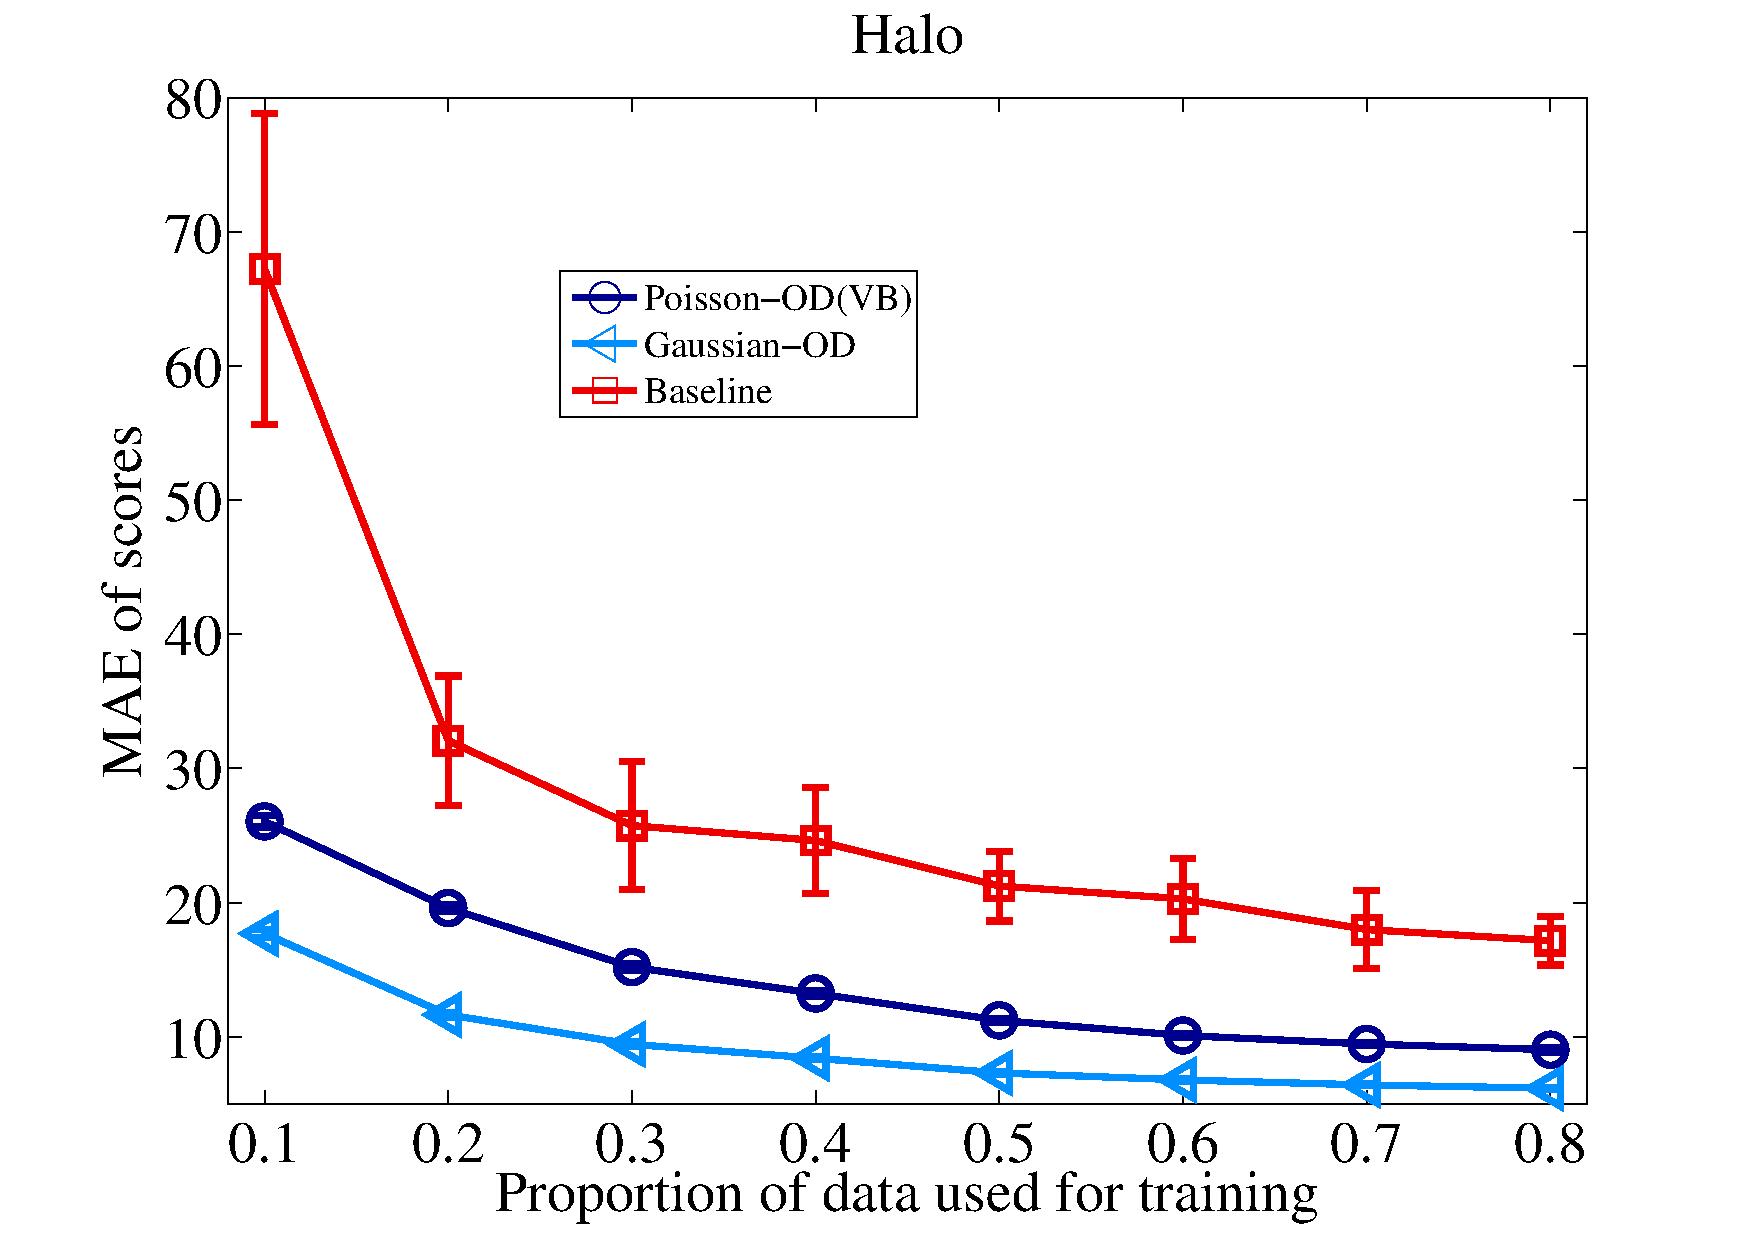
\epsfig{file=ScoreError_Halo, angle=0, height=8cm}
\caption{\small Results on the Halo 2 data set, evaluated using score
prediction error (right column). Error bars indicate
standard errors.}
\label{fig:ScoreError_Halo}
\end{figure*}
\end{center}

%For the results on the Halo dataset, it is interesting to note that the Gaussian-OD and
%Poisson-OD models slightly outperform the Gaussian-SD model. This can
%perhaps be explained by the strength of modeling offence/defence
%skills separately. Note that both the Gaussian-OD and Poisson-OD
%models propose to treat offence and defence skills separately,
%contrasted with the Gaussian-SD model that uses a single skill
%variable.

\COMMENT
By referring to the score
statistics in Table~\ref{table:datasetStatistics}, our {\it
hypothesis} is that {\it the Poisson model is appropriate for
predicting scores when the match outcomes are given as relatively
larger numbers, which can be explained by its exponentiated rate that
allows to amplify small skill differences to predict the correct rates
needed for high scoring games}. Likewise the Gaussian model without
the exponentiation performs better for low scoring games.

In order to verify the hypothesis, we show the estimated skills after
training on the AFL and UK-PL dataset in
Figure~\ref{fig:ResultsEstimatedSKills}. On the AFL data set, the
differences across the skills of different teams learned from the
Poisson model and Gaussian-S are relatively small, which supports the
above hypothesis.

\ENDCOMMENT
% %TODO
% \begin{itemize}
%   \item Table: {\it testing on the last 10 percent data using models learnt from the first 90 percent data; Five by Three (algorithm by datasets);}
%   \item Performance vs. update \#: {\it testing on the last 10 percent data using models learnt from the first ${0.1, \cdots, 0.9}$ portion of the whole data set, for three data set -- 3 figures.}
%   \item Team rankings vs. o+d ranking (parallel lists in a table): {\it AFL and UK-PL give team ranking after each season. I will only evaluate on the team ranking for the last season. Two tables: one for AFL; the other for UK-PL.}
%   \item Score accuracy: {\it Poisson and Gaussian (S) -- score accuracy; Gaussian (SD) -- score difference accuracy;}
%   \item Bar graph predicted/actual win/lose draw: {\it three datasets, five algorithms, plot W/L/D frequency.}
%   \item Rel Info Gain???
% \end{itemize}

\subsection{Poisson-OD(VB) Vs Poisson-OD(Sampling)}
\label{sec:VBSampling}
We studied the performance for the Poisson-OD model when approximate inference is conducted by variational Bayes and slice sampling on the AFL data set. As shown in the various results for three criteria on the AFL data set (Figure~\ref{ScoreError_AFL_without_GaussianOD}), the differences in the performances achieved by the Poisson-OD model with VB and slice sampling are negligible; however, it is important to note that the slice sampling takes about 20 seconds; however, our proposed fixed-point solution often converges after two or three iterations that can be finished within less  than 0.01 seconds. Thus, our proposed variational Bayes inference is much more efficient than the sampling based approaches. For this reason, we can omit the report of the Poisson-OD(Sampling) on other data sets due to heavy computational requirements. Note that one can perhaps explore the advanced sampling approaches such as \cite{Murray:AISTATS2010} to speed up the sampling method. 


% \subsubsection{Model Home Field Improving Performance}
